%==============================================================================
% tento soubor pouzijte jako zaklad
% this file should be used as a base for the thesis
% Autoři / Authors: 2008 Michal Bidlo, 2018 Jaroslav Dytrych
% Kontakt pro dotazy a připomínky: dytrych@fit.vutbr.cz
% Contact for questions and comments: dytrych@fit.vutbr.cz
%==============================================================================
% kodovani: UTF-8 (zmena prikazem iconv, recode nebo cstocs)
% encoding: UTF-8 (you can change it by command iconv, recode or cstocs)
%------------------------------------------------------------------------------
% zpracování / processing: make, make pdf, make clean
%==============================================================================
% Soubory, které je nutné upravit: / Files which have to be edited:
%   xbenes49-20-literatura-bibliography.bib - literatura / bibliography
%   xbenes49-01-kapitoly-chapters.tex - obsah práce / the thesis content
%   xbenes49-30-prilohy-appendices.tex - přílohy / appendices
%==============================================================================
\documentclass[english]{fitthesis} % bez zadání - pro začátek práce, aby nebyl problém s překladem
%\documentclass[english]{fitthesis} % without assignment - for the work start to avoid compilation problem
%\documentclass[zadani]{fitthesis} % odevzdani do wisu a/nebo tisk s barevnými odkazy - odkazy jsou barevné
%\documentclass[english,zadani]{fitthesis} % for submission to the IS FIT and/or print with color links - links are color
%\documentclass[zadani,print]{fitthesis} % pro černobílý tisk - odkazy jsou černé
%\documentclass[english,zadani,print]{fitthesis} % for the black and white print - links are black
%\documentclass[zadani,cprint]{fitthesis} % pro barevný tisk - odkazy jsou černé, znak VUT barevný
%\documentclass[english,zadani,cprint]{fitthesis} % for the print - links are black, logo is color
% * Je-li práce psaná v anglickém jazyce, je zapotřebí u třídy použít 
%   parametr english následovně:
%   If thesis is written in english, it is necessary to use 
%   parameter english as follows:
%      \documentclass[english]{fitthesis}
% * Je-li práce psaná ve slovenském jazyce, je zapotřebí u třídy použít 
%   parametr slovak následovně:
%   If the work is written in the Slovak language, it is necessary 
%   to use parameter slovak as follows:
%      \documentclass[slovak]{fitthesis}
% * Je-li práce psaná v anglickém jazyce se slovenským abstraktem apod., 
%   je zapotřebí u třídy použít parametry english a enslovak následovně:
%   If the work is written in English with the Slovak abstract, etc., 
%   it is necessary to use parameters english and enslovak as follows:
%      \documentclass[english,enslovak]{fitthesis}

% Základní balíčky jsou dole v souboru šablony fitthesis.cls
% Basic packages are at the bottom of template file fitthesis.cls
% zde můžeme vložit vlastní balíčky / you can place own packages here

% Kompilace po částech (rychlejší, ale v náhledu nemusí být vše aktuální)
% Compilation piecewise (faster, but not all parts in preview will be up-to-date)
% \usepackage{subfiles}

% Nastavení cesty k obrázkům
% Setting of a path to the pictures
%\graphicspath{{obrazky-figures/}{./obrazky-figures/}}
%\graphicspath{{obrazky-figures/}{../obrazky-figures/}}

%---rm---------------
\renewcommand{\rmdefault}{lmr}%zavede Latin Modern Roman jako rm / set Latin Modern Roman as rm
%---sf---------------
\renewcommand{\sfdefault}{qhv}%zavede TeX Gyre Heros jako sf
%---tt------------
\renewcommand{\ttdefault}{lmtt}% zavede Latin Modern tt jako tt

\newcommand\tg{\qopname\relax o{tg}}

% vypne funkci šablony, která automaticky nahrazuje uvozovky,
% aby nebyly prováděny nevhodné náhrady v popisech API apod.
% disables function of the template which replaces quotation marks
% to avoid unnecessary replacements in the API descriptions etc.
\csdoublequotesoff

% =======================================================================
% balíček "hyperref" vytváří klikací odkazy v pdf, pokud tedy použijeme pdflatex
% problém je, že balíček hyperref musí být uveden jako poslední, takže nemůže
% být v šabloně
% "hyperref" package create clickable links in pdf if you are using pdflatex.
% Problem is that this package have to be introduced as the last one so it 
% can not be placed in the template file.
\ifWis
\ifx\pdfoutput\undefined % nejedeme pod pdflatexem / we are not using pdflatex
\else
  \usepackage{color}
  \usepackage[unicode,colorlinks,hyperindex,plainpages=false,pdftex]{hyperref}
  \definecolor{hrcolor-ref}{RGB}{223,52,30}
  \definecolor{hrcolor-cite}{HTML}{2F8F00}
  \definecolor{hrcolor-urls}{HTML}{092EAB}
  \hypersetup{
	linkcolor=hrcolor-ref,
	citecolor=hrcolor-cite,
	filecolor=magenta,
	urlcolor=hrcolor-urls
  }
  \def\pdfBorderAttrs{/Border [0 0 0] }  % bez okrajů kolem odkazů / without margins around links
  \pdfcompresslevel=9
\fi
\else % pro tisk budou odkazy, na které se dá klikat, černé / for the print clickable links will be black
\ifx\pdfoutput\undefined % nejedeme pod pdflatexem / we are not using pdflatex
\else
  \usepackage{color}
  \usepackage[unicode,colorlinks,hyperindex,plainpages=false,pdftex,urlcolor=black,linkcolor=black,citecolor=black]{hyperref}
  \definecolor{links}{rgb}{0,0,0}
  \definecolor{anchors}{rgb}{0,0,0}
  \def\AnchorColor{anchors}
  \def\LinkColor{links}
  \def\pdfBorderAttrs{/Border [0 0 0] } % bez okrajů kolem odkazů / without margins around links
  \pdfcompresslevel=9
\fi
\fi
% Řešení problému, kdy klikací odkazy na obrázky vedou za obrázek
% This solves the problems with links which leads after the picture
\usepackage[all]{hypcap}

% Informace o práci/projektu / Information about the thesis
%---------------------------------------------------------------------------
\projectinfo{
  %Prace / Thesis
  project={BP},            %typ práce BP/SP/DP/DR  / thesis type (SP = term project)
  year={2018},             % rok odevzdání / year of submission
  date=\today,             % datum odevzdání / submission date
  %Nazev prace / thesis title
  title.cs={Počítání osob pomocí PIR senzoru},  % název práce v češtině či slovenštině (dle zadání) / thesis title in czech language (according to assignment)
  title.en={Counting People Using a PIR Sensor}, % název práce v angličtině / thesis title in english
  %title.length={14.5cm}, % nastavení délky bloku s titulkem pro úpravu zalomení řádku (lze definovat zde nebo níže) / setting the length of a block with a thesis title for adjusting a line break (can be defined here or below)
  %Autor / Author
  author.name={Martin},   % jméno autora / author name
  author.surname={Beneš},   % příjmení autora / author surname 
  %author.title.p={Bc.}, % titul před jménem (nepovinné) / title before the name (optional)
  %author.title.a={Ph.D.}, % titul za jménem (nepovinné) / title after the name (optional)
  %Ustav / Department
  department={UITS}, % doplňte příslušnou zkratku dle ústavu na zadání: UPSY/UIFS/UITS/UPGM / fill in appropriate abbreviation of the department according to assignment: UPSY/UIFS/UITS/UPGM
  % Školitel / supervisor
  supervisor.name={Martin},   % jméno školitele / supervisor name 
  supervisor.surname={Drahanský},   % příjmení školitele / supervisor surname
  supervisor.title.p={prof. Ing., Dipl.-Ing.},   %titul před jménem (nepovinné) / title before the name (optional)
  supervisor.title.a={Ph.D.},    %titul za jménem (nepovinné) / title after the name (optional)
  % Klíčová slova / keywords
  keywords.cs={Sem budou zapsána jednotlivá klíčová slova v českém (slovenském) jazyce, oddělená čárkami.}, % klíčová slova v českém či slovenském jazyce / keywords in czech or slovak language
  keywords.en={Sem budou zapsána jednotlivá klíčová slova v anglickém jazyce, oddělená čárkami.}, % klíčová slova v anglickém jazyce / keywords in english
  %keywords.en={Here, individual keywords separated by commas will be written in English.},
  % Abstrakt / Abstract
  abstract.cs={
    PIR (pasivní infračervený) senzor se používá zejména pro detekci přítomnosti osoby a oznámení systému pro příslušnou reakci.
    Zaměřením této práce je užití PIR senzorů pro rozpoznávání pozice osoby, rychlosti a směru pohybu nebo počtu lidí ve snímaném prostoru.
    Za tímto účelem je navržen způsob zpracování jeho výstupního analogového signálu, počínající extrakcí příznaků pomocí vlnkové transformace,
    následnou klasifikací a generování výstupu na základě sběru dat z více senzorů pomocí speciálního systému, který ze vstupní matice fuzzy
    čísel generované klasifikátorem pro každý senzor generuje na výstup pozice přítomných osob.

  }, % abstrakt v českém či slovenském jazyce / abstract in czech or slovak language
  abstract.en={
    PIR (passive infrared) sensor are mainly used to detect a presence of a parson and notifying a system to react appropriately.
    The aim of this thesis is to use the PIR sensors to recognize position of person, speed and direction of movement or count of people.
    To do so, thesis suggests a heat signal processing pipeline including wavelet transformation feature extraction, classifier and fuzzy
    logic system, collecting data from multiple sensors, processing them and merging them together into a result.
  }, % abstrakt v anglickém jazyce / abstract in english
  %abstract.en={An abstract of the work in English will be written in this paragraph.},
  % Prohlášení (u anglicky psané práce anglicky, u slovensky psané práce slovensky) / Declaration (for thesis in english should be in english)
  declaration={Prohlašuji, že jsem tuto bakalářskou práci vypracoval samostatně pod vedením pana X...
Další informace mi poskytli...
Uvedl jsem všechny literární prameny a publikace, ze kterých jsem čerpal.},
  %declaration={Hereby I declare that this bachelor's thesis was prepared as an original author’s work under the supervision of Mr. X
% The supplementary information was provided by Mr. Y
% All the relevant information sources, which were used during preparation of this thesis, are properly cited and included in the list of references.},
  % Poděkování (nepovinné, nejlépe v jazyce práce) / Acknowledgement (optional, ideally in the language of the thesis)
  acknowledgment={V této sekci je možno uvést poděkování vedoucímu práce a těm, kteří poskytli odbornou pomoc
(externí zadavatel, konzultant, apod.).},
  %acknowledgment={Here it is possible to express thanks to the supervisor and to the people which provided professional help
%(external submitter, consultant, etc.).},
  % Rozšířený abstrakt (cca 3 normostrany) - lze definovat zde nebo níže / Extended abstract (approximately 3 standard pages) - can be defined here or below
  %extendedabstract={Do tohoto odstavce bude zapsán rozšířený výtah (abstrakt) práce v českém (slovenském) jazyce.},
  %faculty={FIT}, % FIT/FEKT/FSI/FA/FCH/FP/FAST/FAVU/USI/DEF
  faculty.cs={Fakulta informačních technologií}, % Fakulta v češtině - pro využití této položky výše zvolte fakultu DEF / Faculty in Czech - for use of this entry select DEF above
  faculty.en={Faculty of Information Technology}, % Fakulta v angličtině - pro využití této položky výše zvolte fakultu DEF / Faculty in English - for use of this entry select DEF above
  department.cs={Ústav inteligentních systémů}, % Ústav v češtině - pro využití této položky výše zvolte ústav DEF nebo jej zakomentujte / Department in Czech - for use of this entry select DEF above or comment it out
  department.en={Department of Intelligent Systems} % Ústav v angličtině - pro využití této položky výše zvolte ústav DEF nebo jej zakomentujte / Department in English - for use of this entry select DEF above or comment it out
}

% Rozšířený abstrakt (cca 3 normostrany) - lze definovat zde nebo výše / Extended abstract (approximately 3 standard pages) - can be defined here or above
%\extendedabstract{Do tohoto odstavce bude zapsán výtah (abstrakt) práce v českém (slovenském) jazyce.}

% nastavení délky bloku s titulkem pro úpravu zalomení řádku - lze definovat zde nebo výše / setting the length of a block with a thesis title for adjusting a line break - can be defined here or above
%\titlelength{14.5cm}


% řeší první/poslední řádek odstavce na předchozí/následující stránce
% solves first/last row of the paragraph on the previous/next page
\clubpenalty=10000
\widowpenalty=10000

% checklist
\newlist{checklist}{itemize}{1}
\setlist[checklist]{label=$\square$}

\begin{document}
  % Vysazeni titulnich stran / Typesetting of the title pages
  % ----------------------------------------------
  \maketitle
  % Obsah
  % ----------------------------------------------
  \setlength{\parskip}{0pt}

  {\hypersetup{hidelinks}\tableofcontents}
  
  % Seznam obrazku a tabulek (pokud prace obsahuje velke mnozstvi obrazku, tak se to hodi)
  % List of figures and list of tables (if the thesis contains a lot of pictures, it is good)
  \ifczech
    \renewcommand\listfigurename{Seznam obrázků}
  \fi
  \ifslovak
    \renewcommand\listfigurename{Zoznam obrázkov}
  \fi
  % \listoffigures
  
  \ifczech
    \renewcommand\listtablename{Seznam tabulek}
  \fi
  \ifslovak
    \renewcommand\listtablename{Zoznam tabuliek}
  \fi
  % \listoftables 

  \ifODSAZ
    \setlength{\parskip}{0.5\bigskipamount}
  \else
    \setlength{\parskip}{0pt}
  \fi

  % vynechani stranky v oboustrannem rezimu
  % Skip the page in the two-sided mode
  \iftwoside
    \cleardoublepage
  \fi

  % Text prace / Thesis text
  % ----------------------------------------------
  %===============================================================================
% Autoři: Michal Bidlo, Bohuslav Křena, Jaroslav Dytrych, Petr Veigend a Adam Herout 2018

\chapter{Introduction}
\label{chapter:introduction}


Our~body as same as everything surrounding us emits some radiation. The~dominant wavelengths
belong to the~infrared spectrum and our body senses it as a heat. If we pass its significance
for living creatures and the~fact that the~presence of the~right amount of infrared radiation
is essencial for all the~life as we know it, there is also a~lot of usage in the~industry or
generally -- technology.

Infrared waves are used in various devices. From nightvision devices, astronomical telescopes to personal
electronics (infraport, TV remote controller). This thesis focuses on the usage in PIR
sensors -- electronic devices that changes its output based on the amount of received infrared
radiation.

The PIR sensors are used around us a lot even though we might not know it. We all know the waving
of hands towards the~sensor in a~hallway so the light would turn on and we could tie our shoes,
or the~self-opening door in shopping malls or self-rotating door in banks. These mechanisms mostly
use PIR sensors.

\begin{figure}[h!]
  \begin{center}
    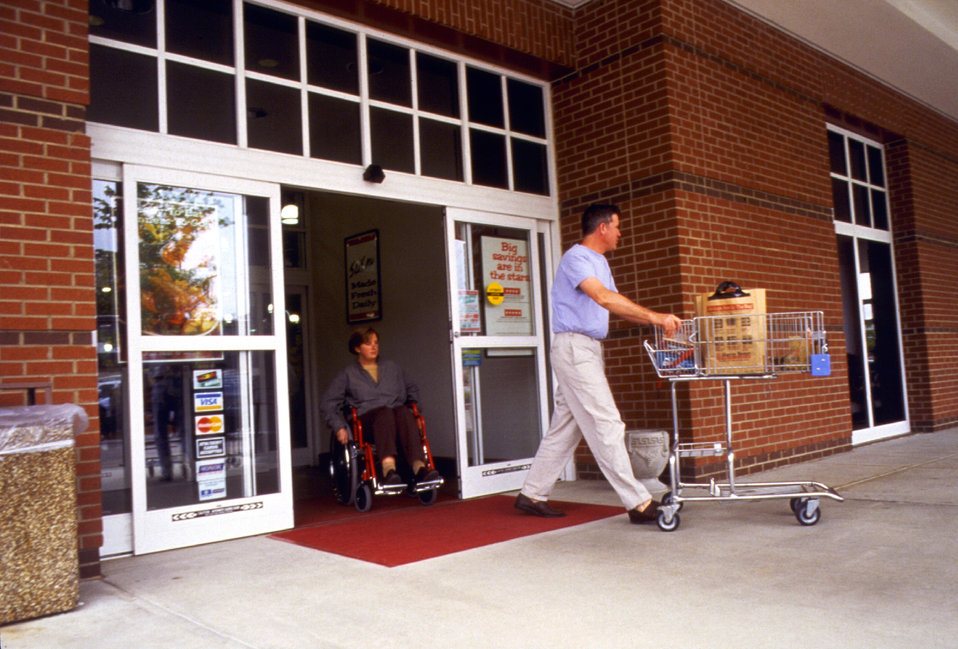
\includegraphics[width=0.5\textwidth]{obrazky-figures/automaticdoorway.jpg}
    \caption{PIR sensor: automatic doorway. \cite{automaticdoorway} \label{fig:automaticdoorway}}
  \end{center}
\end{figure}

PIR sensors offer even more than stating a presence of person. It is possible to~process sensor
output signal to~get more information about~sensed space - a~position of~person, a~number of~people.
Especially when more sensors are used.

The localization using PIR is still matter of intense research, a number of articles has been
written on it. This thesis suggests multisensor attitude and a usage of fuzzy logic to merge
sensor's outputs.



%\chapter{Abstract}
%\label{abstract}
%10 lines 
%Description of problem
%Solution and focus
%Maybe brief conclusion and application







\chapter{State of the art}
\label{theory}


\section{Physics of radiation}

In the~modelled system equations calculating with~infrared radiation are being used -- to~understand
them properly it is necessary to describe what is a~radiation, where does it come from and how can
we measure it. 

As it was already mentioned in the~chapter \ref{chapter:introduction}, every object whose temperature
is higher than absolute zero emits an~electromagnetic radiation.
\begin{equation}
T_{obj}>0~K\equiv -273.15^{\circ}C
\end{equation}
It is caused by a~charged subatomical particles (electrons, protons) that are undergoing an~acceleration,
emitting an~energy in a~form of photon -- electromagnetic radiation.


\subsection*{Characteristics}
The~electromagnetic radiation have a~number of measurable characteristics. The~most significant ones
are {\it frequency} $f$ and {\it wavelength} $\lambda$. Due to the~constant speed of the radiation $v$
aka speed of light $c = v = 3\cdot10^{8}~m\cdot s^{-1}$ not dependent on the frequency, they are
propotional and mutually transferrable.
\begin{equation}
f=\frac{v}{\lambda}=\frac{c}{\lambda}=\frac{3\cdot10^{8}}{\lambda}
\end{equation}

Electromagnetic waves are being divided into categories according to their usage by the wavelength
$\lambda$. With increasing wavelength~$\lambda$ it is gamma, X-rays, ultraviolet (UV), visible light,
infrared (IR) and radio waves. This is called electromagnetic spectrum and it is shown in the image
\ref{fig:spectrum}.

\begin{figure}
\begin{center}
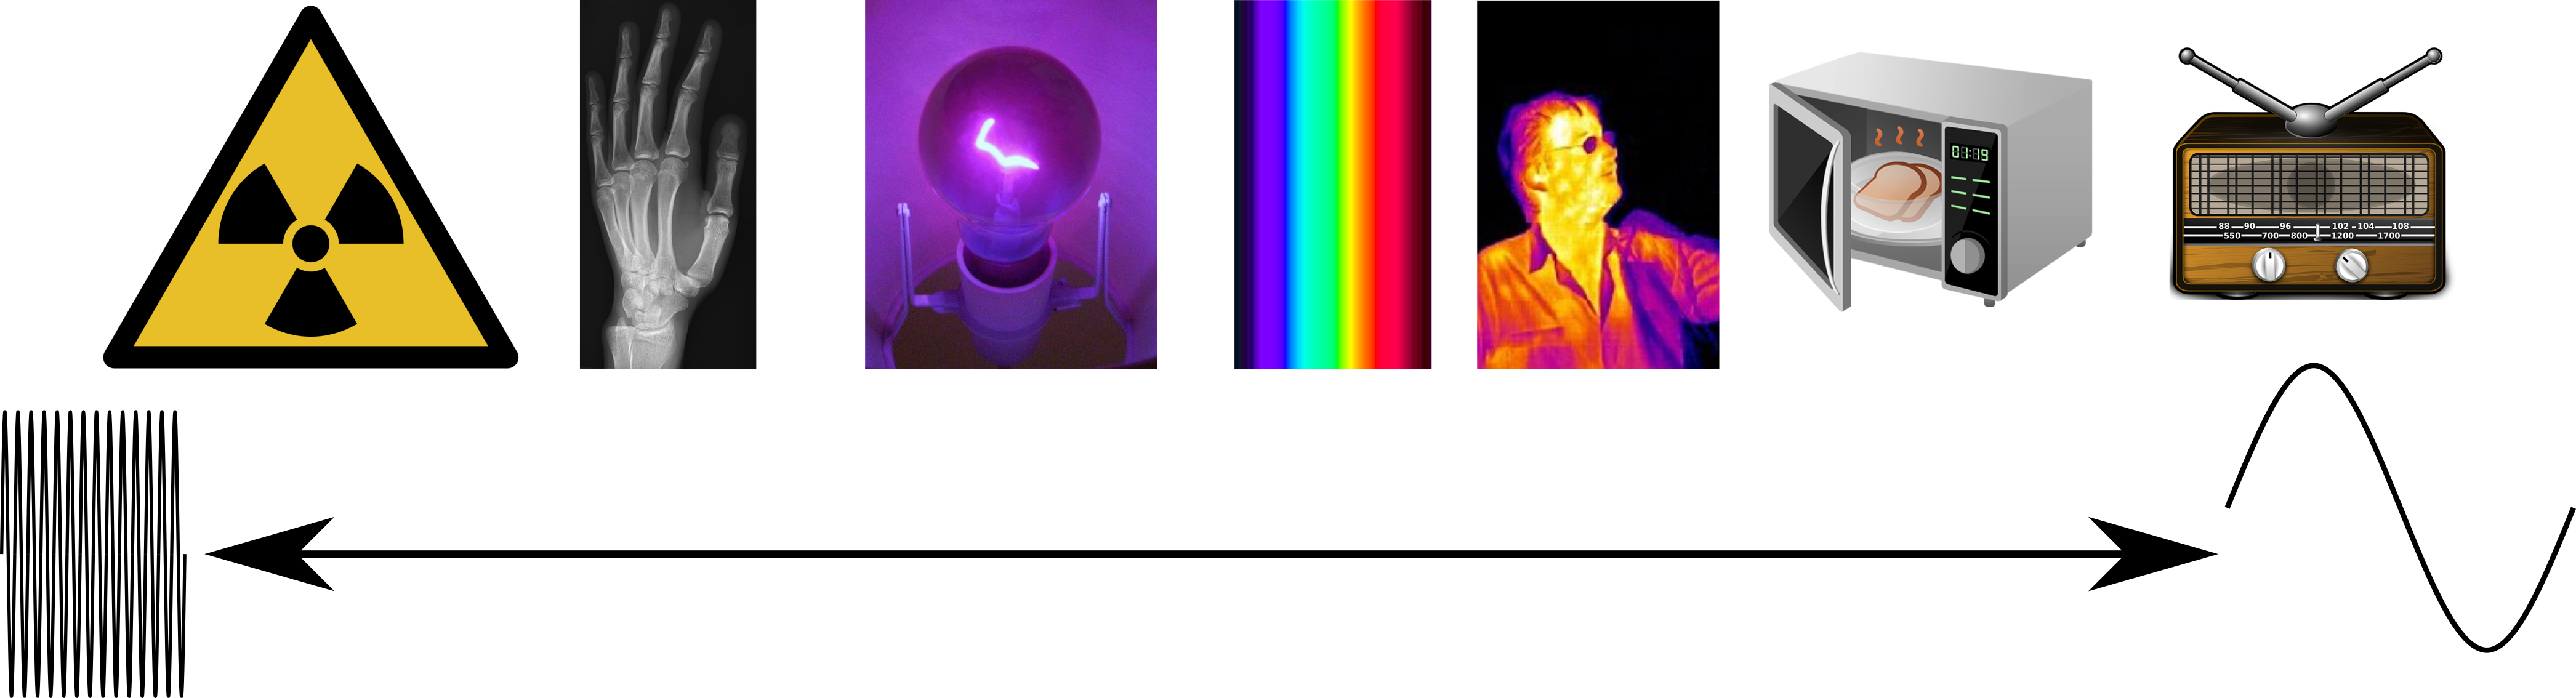
\includegraphics[width=0.8\textwidth]{obrazky-figures/spectrum.png}
\caption{Electromagnetic spectrum.\label{fig:spectrum}}
\end{center}    
\end{figure}

Another measurable characteristic is an~energy of the~radiation $Q$,$E$ or $W$. It is linearly dependend
on its frequency $f$ and can be computed using Planck constant $h=6.63\cdot10^{-34}~J\cdot s $.
\cite{NasaEMSpectrum}
\begin{equation}
W = h\cdot f
\end{equation}

The~power of the~radiation $\Phi$ is called {\it radiant power} or rather {\it radiant flux}. As a~regular
power it is energy per time, since the radiation is four-dimentional, partial derivations must be used.
\begin{equation}
\Phi = \frac{\partial W}{\partial t}
\end{equation}

The radiant power per unit surface is a~flux density. It is called either {\it radiant exitance} $M$
when emitting or {\it irradiance} $E$ when receiving.
\begin{subequations}
\begin{equation}
M = \frac{\partial \Phi_{emitted}}{\partial S_{sender}}
\end{equation}
\begin{equation}
E = \frac{\partial \Phi_{received}}{\partial S_{receiver}}
\end{equation}
\end{subequations}
The~Stefan-Boltzmann law defines irradiance of electromagnetic radiation as
\begin{equation}
I = \sigma \cdot T^4
\end{equation}
where $\sigma = 5.6704\cdot 10^{-8} Wm^{-2}K^{-4}$ is the~Stefan-Boltzmann constant and $T$ is a~thermodynamic
temperature.

Power per unit solid angle $I$ is called {\it radiant intensity}. With dividing by an~area of the~item
projected from certain direction we get an~amount of power emitted in that~direction called {\it radiance} $L$.
\begin{subequations}
\begin{equation}
I = \frac{\partial \Phi}{\partial \Omega}
\end{equation}
\begin{equation}
L = \frac{\partial I}{\partial S cos(\theta)}
\end{equation}
\end{subequations}
Other characteristics of radiation can be seen in the~table \ref{table:units}. \cite{iso800007} \cite{TemperatureMeasuring}

\begin{table}
\begin{tabular}{|c|c|c|l|} \hline
\textbf{Name}             & \textbf{Symbol} & \textbf{Unit}                 & \textbf{Definition}                             \\ \hline
Radiant flux        & $\Phi$          & $W$                           & Power transfered by a radiation.                \\ \hline
Radiant exitance    & $M$             & $W\cdot m^{-2}$               & Sent $W$ per sender's surface.                  \\ \hline 
Irradiance          & $E$             & $W\cdot m^{-2}$               & Received $W$ per receiver's surface.            \\ \hline
Radiant intensity   & $I$             & $W\cdot sr^{-1}$              & $W$ per unit solid angle.                       \\ \hline
Radiance            & $L$             & $W\cdot sr^{-1}\cdot m^{-2}$  & $I$ per sender's area projected to a direction. \\ \hline
\end{tabular}
\caption{Radiation characteristics.\label{table:units} \cite{TemperatureMeasuring}}
\end{table}



\newpage
\section{Temperature homeostasis}
The animal bodies require physical and chemical conditions in order to work properly (or at all). One of
the physical aspects is a temperature. There are generally three types of animals -- {\it ectotherms},
{\it endotherms} and {\it mesotherms}.

Ectotherms do not regulate its body temperature and rely on an external source, endotherms keeps it
constant independently on the environment, so called {\it homeothermy}\footnote{Homeothermy is an aspect
of homeostasis. It means keeping its inner body temperature within the preset limits.}. Mesotherm
strategy is then something in between.

Endotherm groups are birds and mammals, the most significant ectotherm group are reptiles. They compensate
it with basking in the sun. The thermal characteristics of these groups can be seen in the figure \ref{fig:thermoregulatory}.

\begin{figure}[h!]
\begin{center}
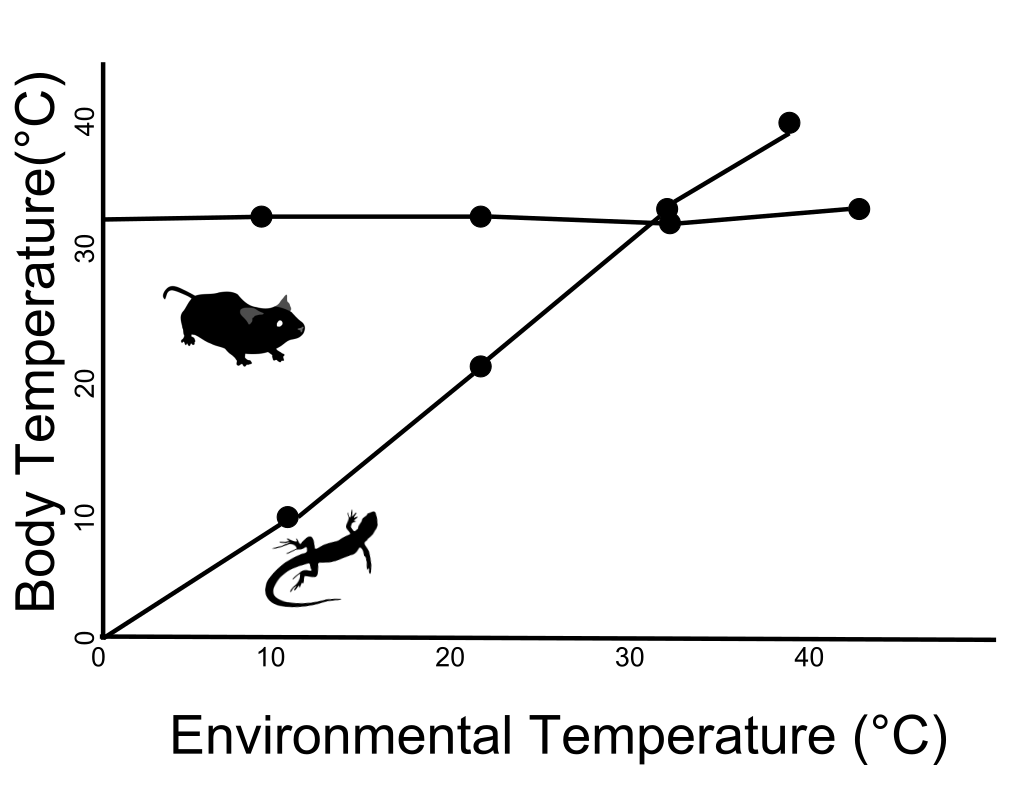
\includegraphics[width=0.4\textwidth]{obrazky-figures/thermoregulatory.png}
\caption{Thermal regulation graph.\label{fig:thermoregulatory}\cite{thermoregulatory}}
\end{center}    
\end{figure}

Human body temperature $T_{HB}$ varies in $\langle 36^{\circ}C; 38^{\circ}C \rangle$, in the hyperthermia
it can rise up to $40^{\circ}C$. The figure \ref{fig:bodywavelength} shows the radiation wavelength composition.
The peak wavelength (temperature $37^{\circ}C$ or $310.15~K$) can be calculated with the Wien's displacement law.
\begin{equation}
\lambda_{max}=\frac{b}{T}=\frac{2.8977729 \cdot 10^{-3}}{310.15} = 9.3431~\mu m
\end{equation}

\begin{figure}[h!]
\begin{center}
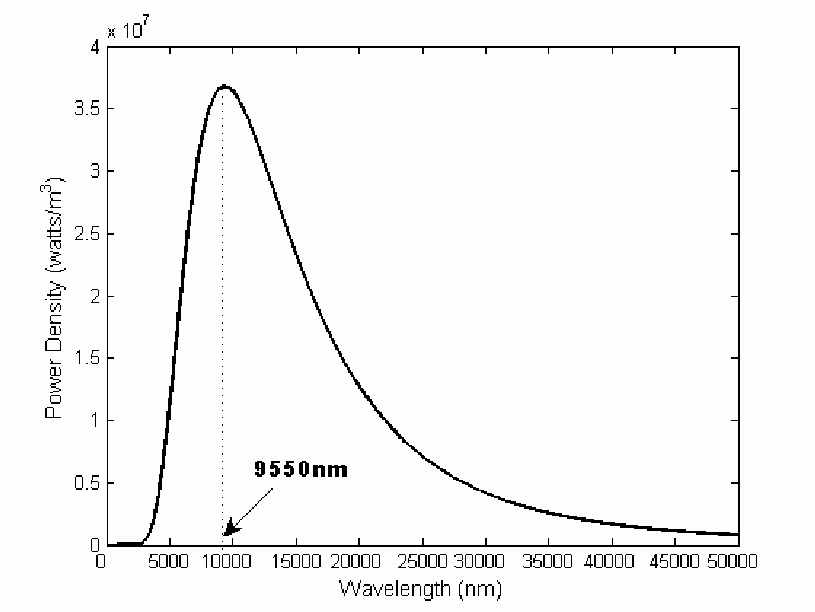
\includegraphics[width=0.4\textwidth]{obrazky-figures/bodyradiation.png}
\caption{Human body radiation wavelength.\cite{BodyRadiation}\label{fig:bodywavelength}}
\end{center}    
\end{figure}





\newpage
\section{Radiation perception}

\subsection*{Radiation processed by organisms}
This~thesis describes a~particular way how to use the~infrared radiation. Very important beginning of such
work is always studying existing applications. Unforgettable one is a~nature -- how evolution enabled 
various organisms to~use it.

Many animals can process parts of electromagnetic spectrum. Eyes enables mammals, cephalopods and arthropods
to sense a visible light, some insects can even see a~part of UV. Additionally organisms including human often
have thermoreceptors in~their skin so they can get information about intensity of infrared radiation around them.


\paragraph{Visible light}
\label{subsection:eye}
PIR~sensor structure is obviously inspired by a~human eye. Human eyes can process radiation
$\lambda \in \langle 380~nm;760~nm \rangle$ called visible light, one of the~bands of an~electromagnetic spectrum.
Seeing means receiving a light from a~light source reflected by the~surface of an~observed object to our retina.
A~biological system composed of~light-sensitive cells {\it rods} and {\it cones} propagates the~information
through nerves to brain.

A~ray coming to an~eye is going through a~converging lens, which changes its~trajectory aiming to~the~retina,
in~the~best case to~the~most sensitive place with a~lot~of~the~rods and cons called {\it Fovea~centralis}.
\cite{LightEyeVision}

\begin{figure}[h!]
\begin{center}
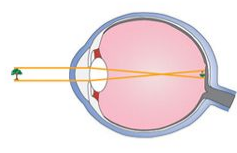
\includegraphics[width=0.3\textwidth]{obrazky-figures/eye.png}
\caption{Structure of an eye. \cite{Eye}\label{fig:eye}}
\end{center}    
\end{figure}


\paragraph{Heat}
The~infrared rays surrounds us during our whole life, we sense it as~heat. The~heat receptors called
{\it thermoreceptors} in our body are located on its~surface (in the~skin), but also in~organs.
The~structure of~a~skin is shown in the figure \ref{fig:skin}. 

There is a~difference between sensing a~visible light and an~infrared radiation. Visible light comes
mostly reflected from the surface, while the IR can originate only from the~primary source -- warm item.

Our skin contains two types of~thermoreceptors: sensing cold, colder than a~body temperature and
hot, hotter than a~body temperature. The~skin structure is shown in~the~figure \ref{fig:skin}.
This is already well described, on the~other hand the~evaluation center of~these receptors in~the~brain
and its~mechanisms is~not fully understanded yet and a~matter of current research. \cite{BodilySenses}

\begin{figure}[h!]
\begin{center}
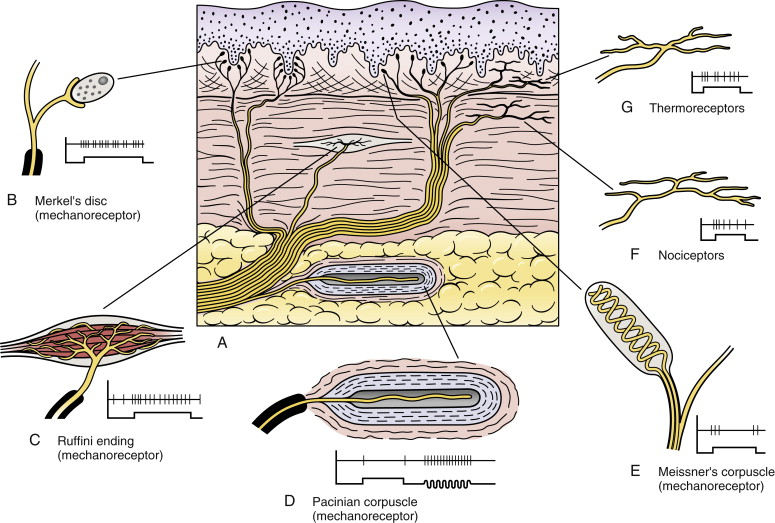
\includegraphics[width=0.45\textwidth]{obrazky-figures/skin.jpg}
\caption{Structure of a~skin. \cite{SkinStructure}\label{fig:skin}}
\end{center}    
\end{figure}

Some animals even use sensing the heat as~a~primary way how to~survive. Several groups of~snakes
(pythons, rattlesnakes, boas and others) use it when hunting warm-blooded animals (mouses, rats, rabbits etc.).
Blood-eating organisms (vampire bats, south-american heteroptera {\it Triatoma infestans})
have IR receptors to~look for a~vein under the skin.\cite{SnakeInfrared}


\paragraph{Discovery}
For the~first time, the~infrared electromagnetic waves were observed and named in 1800 by German-English
astronome sir Frederick Harschel. He dispersed light by a~prism and found out that the~temperature
of~the~light is growing with wavelength, the~red light had the~highest one.

When he measured the~temperature behind the red light, there was no~visible light on~the~table but
the~thermometer was showing even higher temperature moving beyond~the~red spectrum. Harshel
pronounced hypothesis that except the~visible light there must be also invisible one which we can~not
see. \cite{HerschelLife}

%\begin{figure}[h!]
%\begin{center}
%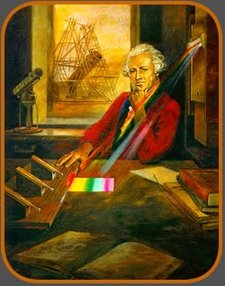
\includegraphics[width=0.4\textwidth]{obrazky-figures/herschel.jpg}
%\caption{Sir William Herschel discovering the~infrared radiation.\cite{HerschelLife}\label{fig:herschel}}
%\end{center}    
%\end{figure}

A~great coincidence is that he was an~astronome, he even discovered the~planet Uran, and it is his discovery,
the~IR waves, which now enables us to~explore and understand the~universe. \cite{NasaIrVideo}



\subsection*{Infrared radiation processed by machines}
\label{IRsensing}
PIR ({\it passive infrared}) sensor is an electronic device that scans electromagnetic
radiation at~wavelength $\lambda\in \langle 700~nm;2.5~mm \rangle$ aka frequency $f\in \langle 120~MHz;430~THz \rangle$. \cite{an2105}

\paragraph{Principles of PIR sensor}
There is a~number of approaches how to~construct such a~sensor. The~point is to~convert the electromagnetic
energy in~electric voltage and send it away via wire to~be processed by~hardware or~software.

First way how to do it is {\it a~bolometer}. It uses the fact that resistance of a~resistor is different
when changing a~temperature, as shown in the equation \ref{eq:bolo} for temperature difference $\Delta T$
and resistor with original resistance $R_0$ and new resistance $R_t$ and with temperature coefficient $\alpha$.
So with using the~same voltage it measures the~electric current and with the~Ohm law $R = \frac{U}{I}$
the~sensor computes instantaneus resistance.

\begin{equation}
\label{eq:bolo}
R_t = R_0 (1 + \alpha\Delta T)
\end{equation}

Another type is {\it a thermoelectric sensor} reacting to the different thermoelectric resistance of
exposed wire and comparative wire.

The~last is {\it a~pyroelectric detector}. The~principle is based on~electrostatic polarization,
changing during the~temperature change. \cite{DetectorsBook}

\begin{figure}[h!]
\begin{center}
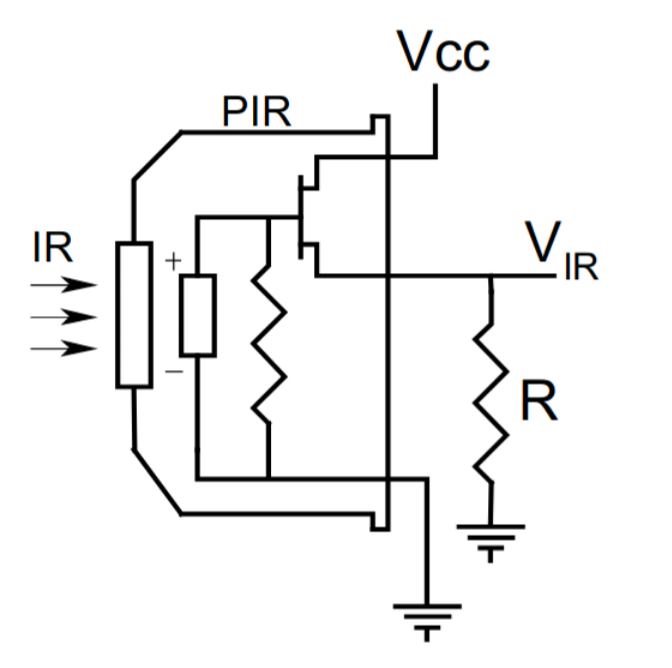
\includegraphics[width=0.25\textwidth]{obrazky-figures/pirscheme.png}
\caption{Single element pyroelectric detector.\cite{an2105}\label{fig:pir}}
\end{center}    
\end{figure}


\paragraph{Sensing of the infrared radiation}
The~structure of~PIR sensor is inspirated by structure of an~eye described in~subsection \ref{subsection:eye}.
An infrared ray incoming to the~sensor first goes through~{\it Fresnel lens} aiming it onto~a~pyroelectric sensor
as you can see in the~figure \ref{fig:fresnellens}. Then the~ray is transformed in an~electric voltage.

\begin{figure}[h!]
\begin{center}
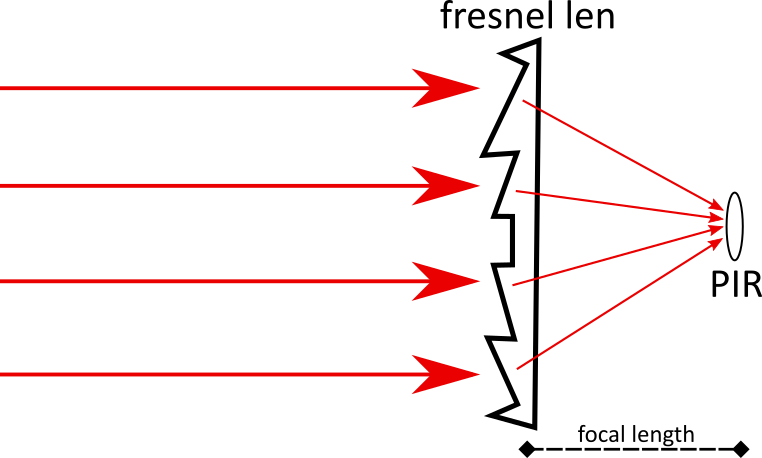
\includegraphics[width=0.3\textwidth]{obrazky-figures/fresnellens.png}
\caption{Fresnel lens.\label{fig:fresnellens}}
\end{center}
\end{figure}

Before the output the signal is being processed. For vast majority of application we are interested in
people sensing emitting radiation characterized in the figure \ref{fig:bodywavelength}.
Therefore the signal is amplified and filtered to well discriminate their presence and absence.
An example is a scheme \ref{fig:pirstd} of product {\it PIR STD} made by {\it B+B Sensors}.

\begin{figure}[h!]
\begin{center}
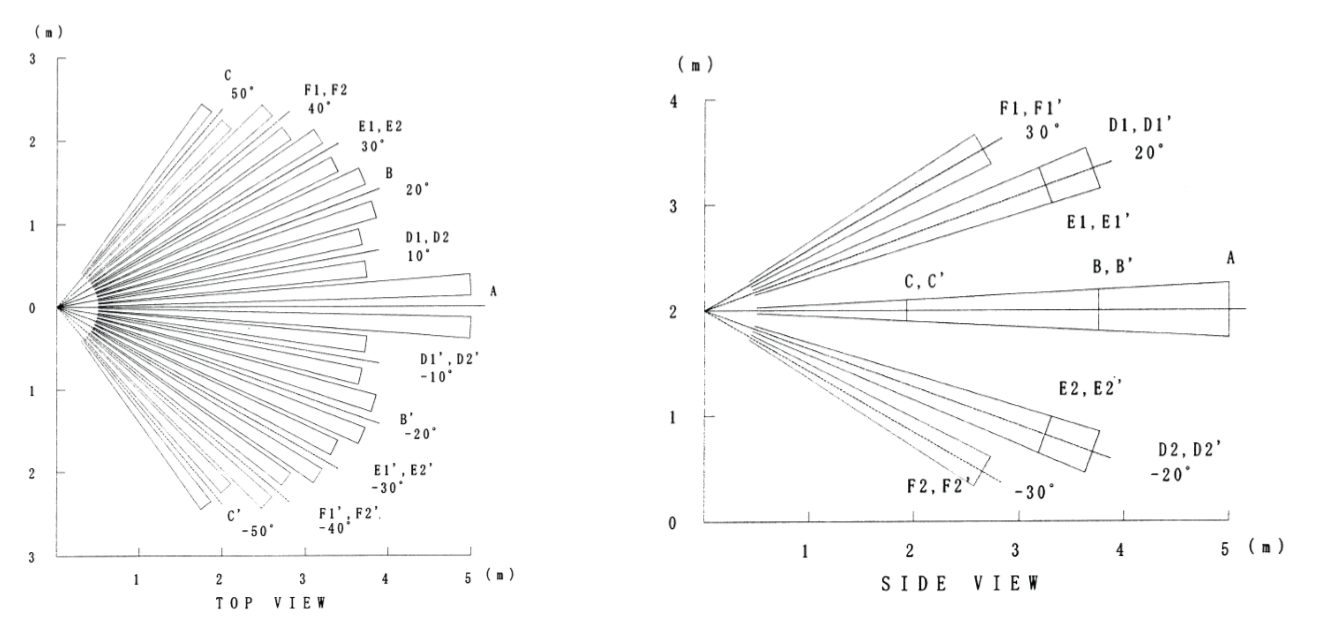
\includegraphics[width=0.7\textwidth]{obrazky-figures/roomsegments.png}
\caption{Sensing of PIR STD. \cite{PIROperationalManual}\label{fig:roomsegments}}
\end{center}    
\end{figure}



\newpage
\section{Pattern recognition}
The pattern recognition means processing of a signal and localizing of predefined objects.
The form is dependent on the type of signal and the objects that we search. Generally we can say
there are five parts of recognition pipeline.

\subsection*{Sensing}
In the world of digital computers sensing means {\it sampling}, converting a continuous signal
into discrete samples. It is present if the signal is being processed online.

Through different signal types various technologies for sensing are used -- image, sound, temperature,
pressure, weight, smell etc. The sensing procedure in the case of heat signal is described in the section
\ref{IRsensing}.

There is a few things that we need to deal during sensing: noise, linearity, callibration, ageing.

\subsection*{Segmentation}
The signal is splitted into segments by the time axis that are being processed separately. They can even overlap.
Segmentation ensures fast processing saving memory and other resources.

\subsection*{Features extraction}
Features are quantitive expression of the input signal, they replace the signal in the following phases.
Its purpose is to reduce memory and computational complexity of the processing. Each segment of $N$ samples
is transformed to vector of $K$ features, the point is to reduce dimensions, $K << N$, but preserve
relevant characteristics. Choosing the right features is therefore key for the following classifier.

To have good results the~features should be discriminative (distinguish between classes), invariant to
the transformations (translation, rotation, scale, deformation etc.) and decorrelated - mutually independent.

Vast number of described ways how to create features exists -- {\it Principal Component Analysis} (PCA),
{\it Linear Discriminant Analysis} (LDA). They can be used generally, but there is also many special
application-dependent features. 

\begin{figure}[h!]
\begin{center}
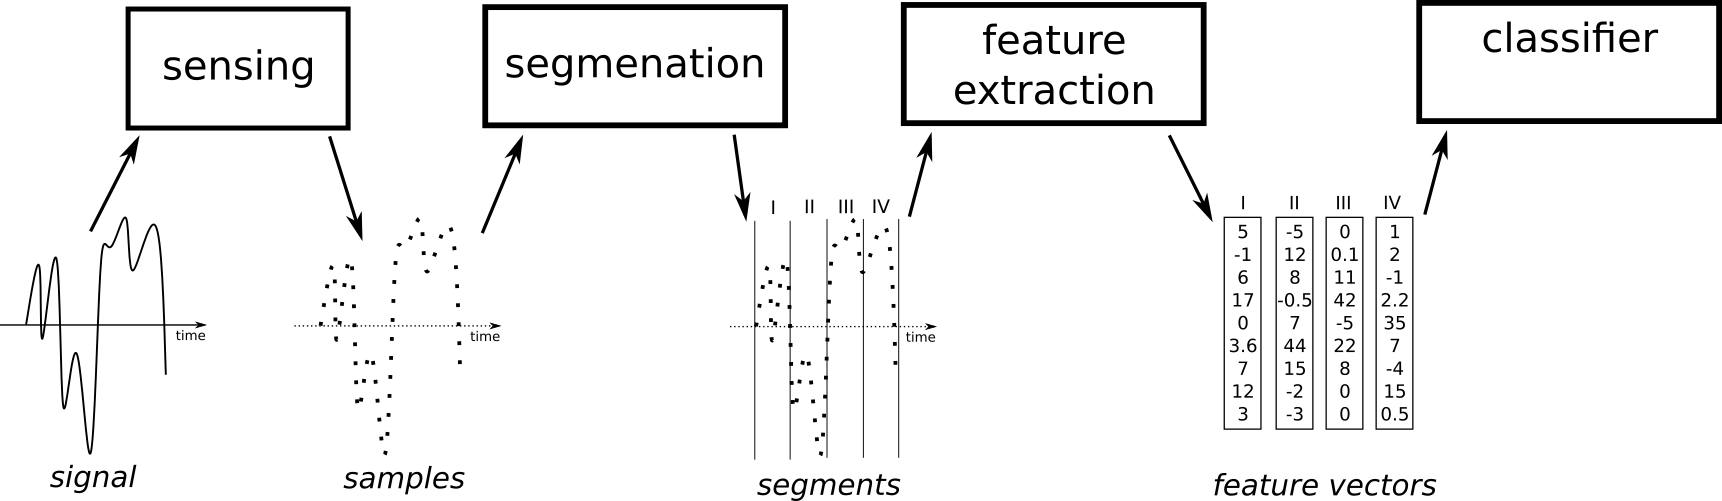
\includegraphics[width=0.7\textwidth]{obrazky-figures/featureextraction.png}
\caption{Preprocessing pipeline.\label{fig:featureextraction}}
\end{center}
\end{figure}

Multiple thesis and articles were written on the topic of heat signal processing. For the feature extraction,
\cite{SinglePIR} suggests {\it Wavelet Transformation}, \cite{ChirpletSVM} uses {\it chirplet}-based features,
but also tests other feature-extraction methods: PCA, Expanded-Class LDA or fusion of PCA and LDA feature vectors,
\cite{BayesanClassifier} calculates with the signal itself.

\subsection*{Classification}
Before we will describe the classification phase, several terms must be defined: 
\begin{itemize}
\item {\it Detection} is a~classifying of presence of observed object or~characteristic.
\item {\it Identification} is an~assigning the~observed object to~one of~$N$ classes.
\item {\it Detection Error Tradeoff} is a~relation of~miss to~false alarm probability of~a~classifier.
The~goal is minimizing both with finding the~best settings of~classifier parameters.
\end{itemize}
This thesis performs a detection of~a~presence of~a~person. In~the~case of~positive detection identification
of~the~situation is made -- what was actually detected and whether it is a~person or more people etc.

Finding the~most suitable classifier for~the~task is fundamental, but consequent to the~feature extraction
method we use. At~the~end of~the~day, inputs of~all the~methods is a~vector of~features for~each segment.
There are linear and non-linear classifiers, separating the~hyperdimentional space into~segments. Then
the~segment is detected or identified if features vector geometrically lies in~the right segment. 

It is also possible to~perform some kind of transformation before classification if the~space is not separable
linearly. But other attitudes are also possible like algorithm {\it K-nearest neighbors}.

An~output of a~classifier can be either a~hard decision or some~kind of soft score, which can be later processed
by a~postprocessor -- used to merge data from~more classifiers or something else. A~classical linear classifier
is used in {\it Linear Regression} or {\it Support Vector Machine} (SVM). Each neuron of recently very popular
{\it Neural Networks} (NN) can also be represented with linear classifier.

\begin{figure}[h!]
\begin{center}
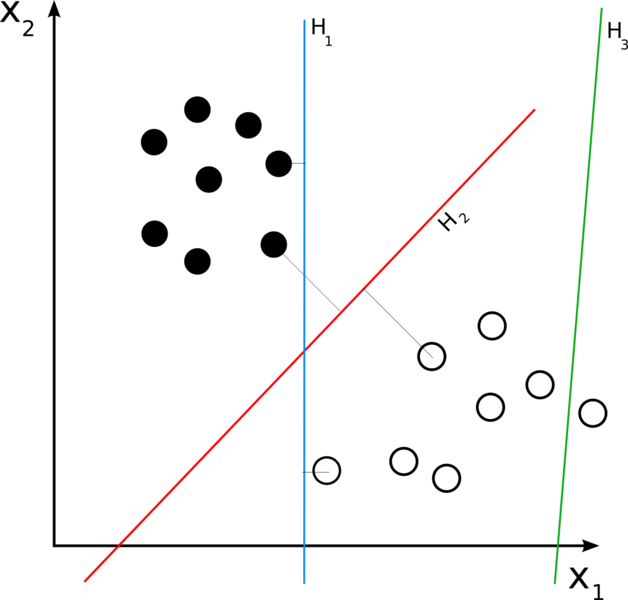
\includegraphics[width=0.3\textwidth]{obrazky-figures/linear.png}
\caption{Linear classifier.\cite{LinearClassifier}\label{fig:linearclassifier}}
\end{center}
\end{figure}

\subsection*{Postprocessing}
During postprocessing different information than pattern are used, procedure is
connected to the concrete task. This parts often includes hard decision, if the
classifier's output is a soft score -- prices are taken into consideration,
the simpliest way is using treshold.




\chapter{Design Description}

The design of the whole project is split in two products - sensing device
and the processing and visualising program - a server. Sensor measures signal
sensing the observed space with connected PIR sensor and sends the data. The server
collects the data from the sensor/sensors and performs the recognition of 
people and fusion algorithms over the results, if multiple sensors are connected.

Results might be displayed in the visualization program. The data are being sent
over network. In the implementation, LAN is used, but it could be possible to
use the Internet and send the data to the remote visualizer.


\section{Sensor device}

Heart of the sensing device is a preprogrammed MCU with PIR connected. Such device
uses AD convertor to read the signal value from the sensor. The device may also
perform fixed-sized segmentation in order to increase the effective data speed with
sending more samples within one chunk, but with regard to preserving {\it real-time}
nature.

One of the great issues, that needs to be solved is determining the position of the sensor,
or even worse -- mutual position of multiple sensors when used. Unless it is
known, no fusion can be done. If the intention is to sense the door area and count
number of incoming/outgoing people, then a position of the door needs to be known
in advance.

Very elegant solution is suggested in \cite{GestureControl}. Three PIR sensors are
places in fixed mutual position on a board, as shown in the figure \ref{fig:3pir_geometry}.
This brings several advantages, not only it increases the sensing angle,
but also solves problems with position of sensors, which is given by the board construction.
Such a construction is unsuitable to use in rooms though.

\begin{figure}[h!]
\begin{center}
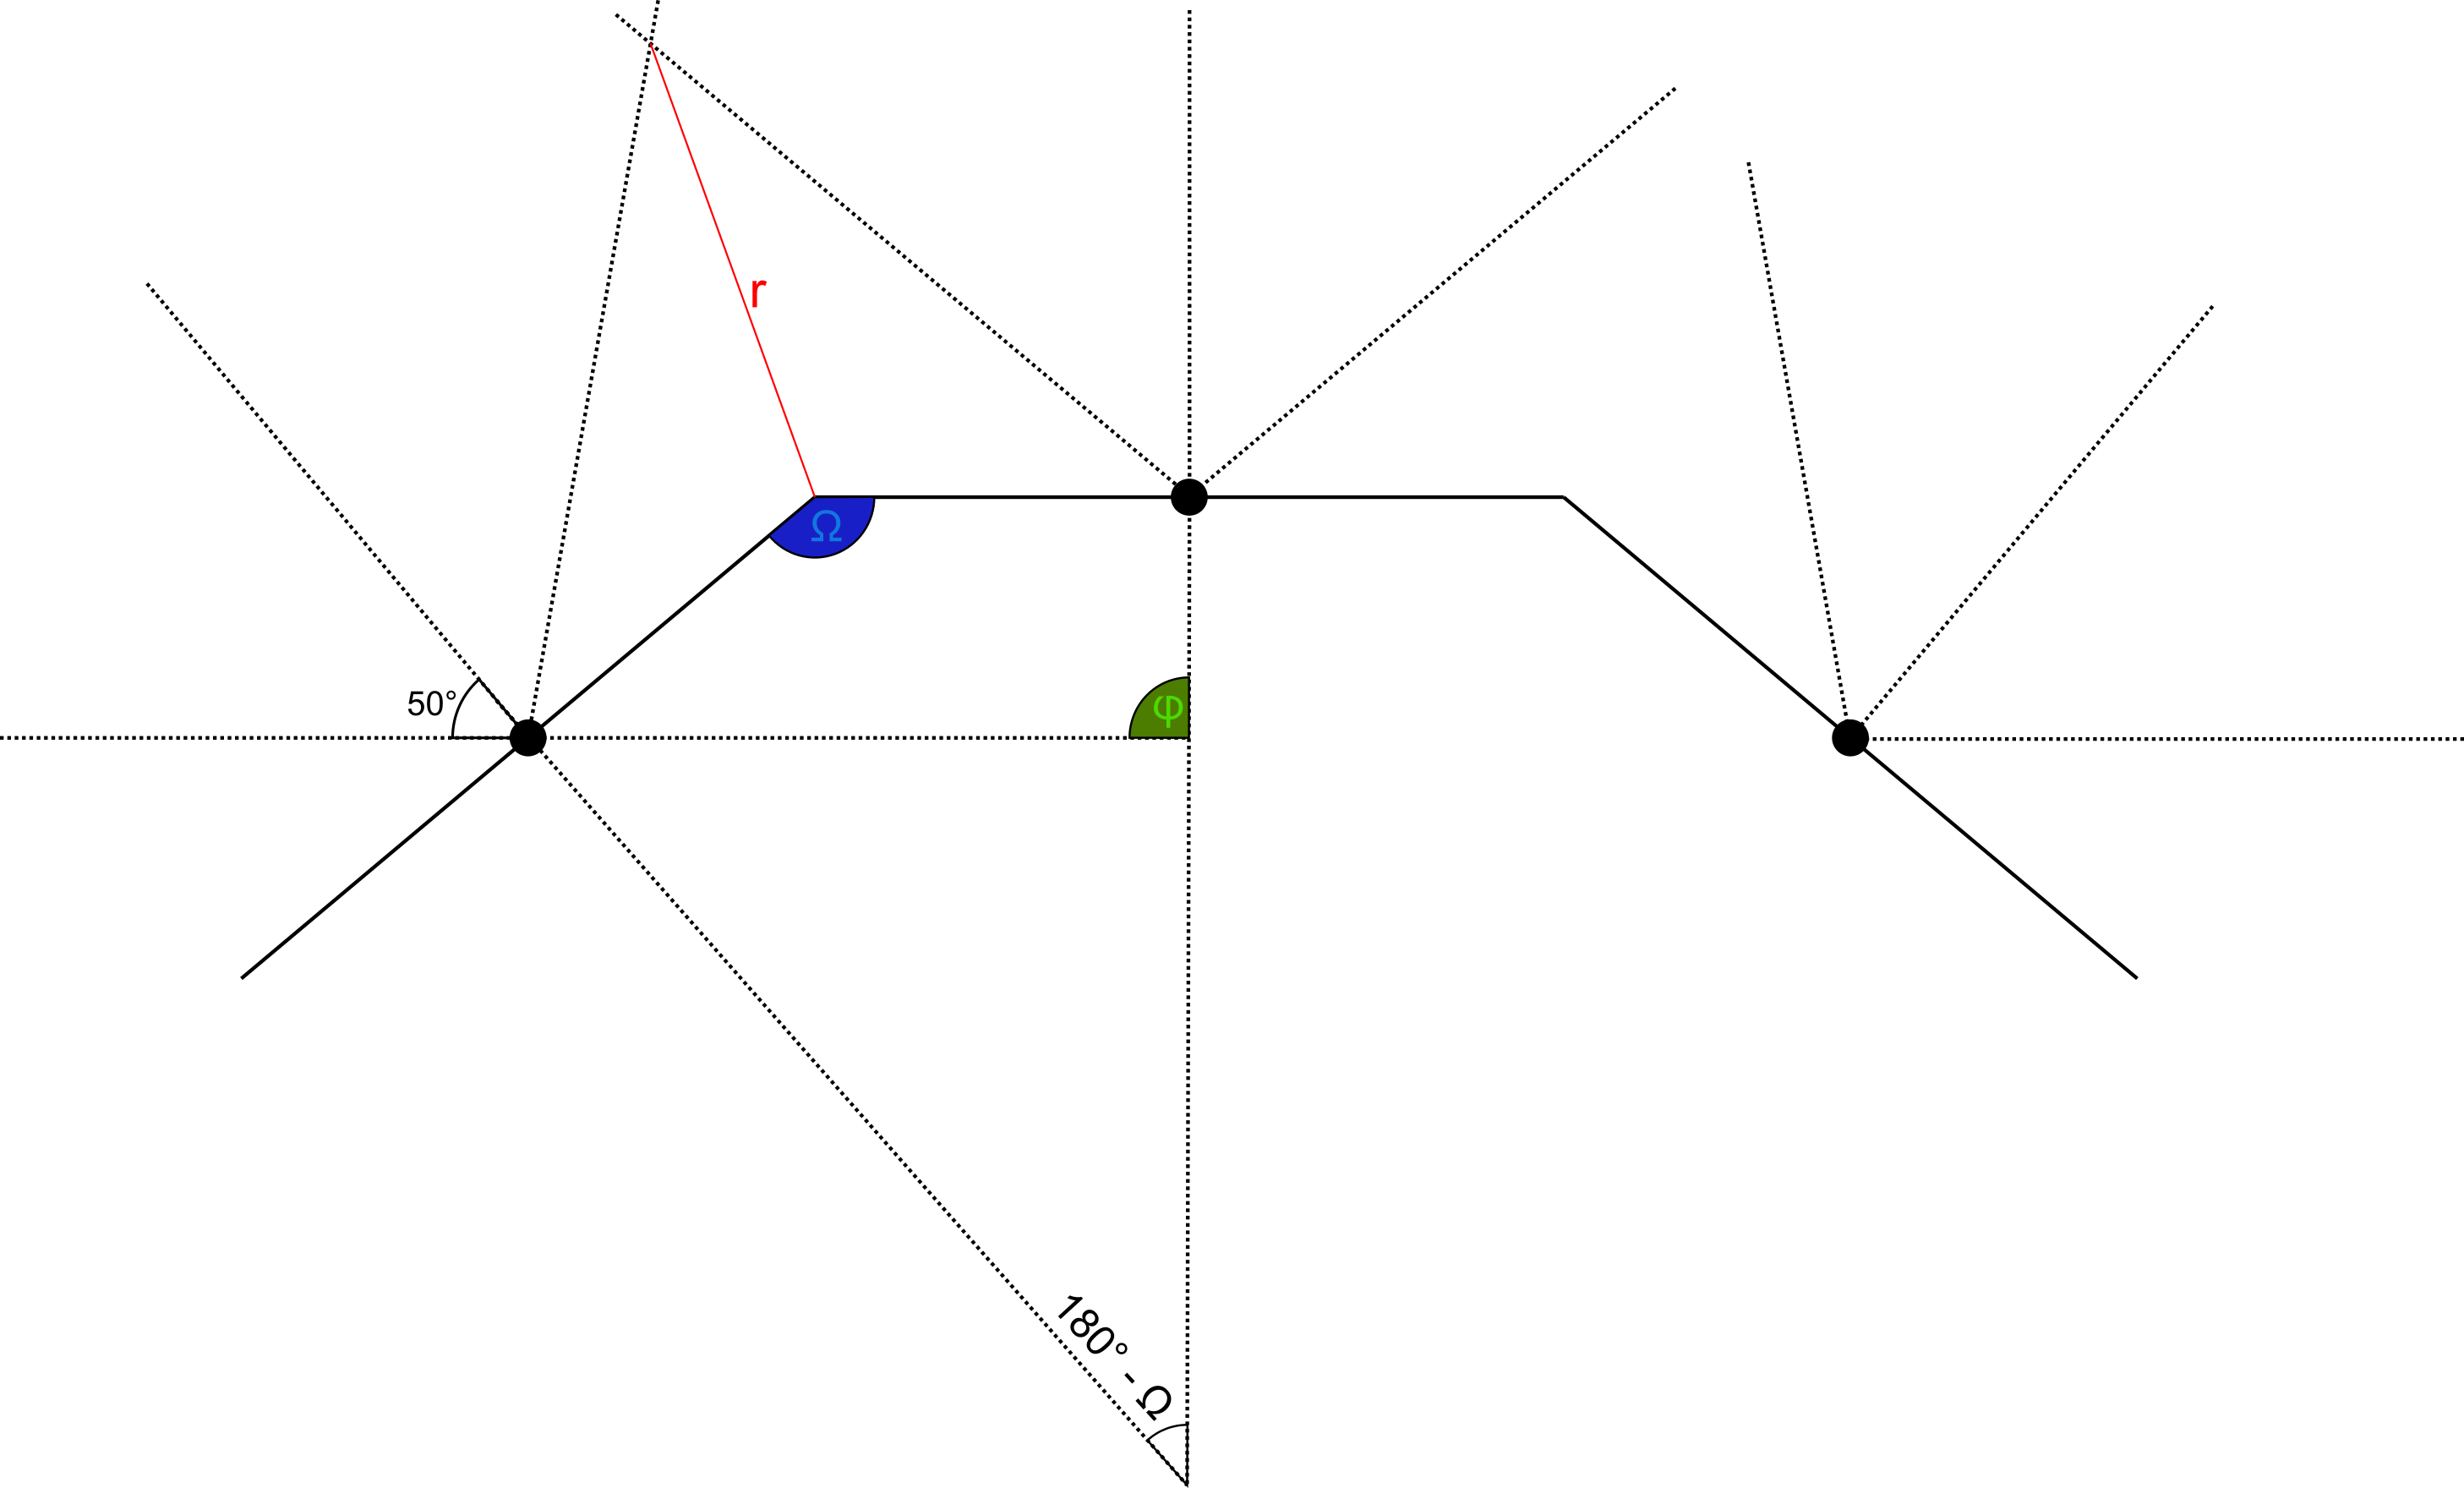
\includegraphics[width=0.4\textwidth]{obrazky-figures/3pir_geometry.png}
\caption{Geometry for three PIR sensors.\label{fig:3pir_geometry}}
\end{center}
\end{figure}

More flexible solution is probably inserting the dimension of space measured by the sensors
and their position directly to the fusion app as parameters. Issue of this is the positioning
itself. On the other hand, this solution can be easily extended with more parameters:
position of doors that can persons come or leave, windows and heaters that can have
unwanted influence and many others.

The device uses a serial communication channel, that can be read by the server. To
increase effectivity of the communication, the MCU sends the data in fixed period
as the chunk of fixed number of samples. The right size of the chunk must be chosen
with regard to the effectivity, but keeping the reaction fast enough. Sampling period and
sending period could be changed in the MCU configuration using REST API if the MCU
is reachable in a network and keeps a running web server.



%classification process described in subsection \ref{label:dataprocessing}.

%The sensors signal is at the end fused together and the results are classified objects
%with coordinates in polar coordinate system relative to the module position. These
%coordinates are sent to the client.

%The interior angle of module $\Omega$ is a parameter of the module construction. Using this parameter
%orientation $\lambda$ and position $p_X = (d_X,\varphi _X)$\footnote{Position uses polar coordinates
%with the origin in the central sensor.} of sensors can be expressed. Parameter $r$ is length
%of module edges with sensor in the center. Sensor PIR-STD by B+B Sensors has $250\times 250\times 200~\text{mm}$;
%therefore $r > 250~\text{mm}$.

%\begin{subequations}
%\begin{equation}
%\lambda_C = 0
%\end{equation}
%\begin{equation}
%\lambda_L = -\lambda_R = 180 - \Omega
%\end{equation}
%\end{subequations}

%\begin{subequations}
%\begin{equation}
%\varphi_C = 0
%\end{equation}
%\begin{equation}
%\varphi_L = -\varphi_R = 90 + \frac{180 - \Omega}{2}
%\end{equation}
%\end{subequations}

%\begin{subequations}
%\begin{equation}
%d_C = 0
%\end{equation}
%\begin{equation}
%d_L = d_R = \frac{r}{2} (r - 4cos(\Omega))
%\end{equation}
%\end{subequations}


\section{Classification server}
\label{section:classification}
On the used communication medium is running application listening to the channel.
This server parses the segments sent by the devices and performs the classification.


\subsection*{Artefact extraction and fuzzification}
The signal produced by the PIR has a specific nature, as it is shown in the appendix \label{appendix:PIRSignal}.
There are parts, that are constant, divided by abruptly changing edges, when there is a moving body. The
characteristics of the movement change character of the signal.

The signal first is segmented using {\it continuous wavelet transformation}
\footnote{
Continuous wavelet transformation is a signal processing technique transforming a signal to frequency domain.
The process is quite similar to fourier tranformation, instead of sinusoid it uses wavelet, a finite signal with
energy $E=0$, and therefore reacts better to abrupt changes.\cite{WaveletTour}}
with Morlet wavelet (\ref{eq:morlet})
and scale $s_{cwt} = 1.33846$, and the extrems are detected comparing to the $N_{n} = 8$ neighbors on both sides.
Detected extrems are used as the borders of the segments, that lies in between them. These numbers were
discovered experimentally minimizing the sum of the within-segment variances of the recorded data using formula \ref{eq:cwtparamssearch}



% Morlet "mexican hat" wavelet.
\begin{equation}
\Psi(x) = e^{-\frac{x^2}{2}} cos(5x)
\label{eq:morlet}
\end{equation}

% Experimental optimalization of parameters.
\begin{equation}
s_{cwt}, N_{n} = \text{argmin} ( \sum_{\sigma_i \in \sigma_{s,N}} \sigma_i )
\label{eq:cwtparamssearch}
\end{equation}

In the next step segment distances are evaluated. Distance of two adjoining segments aka {\it edge} is computed as numerical
difference of their within-segment mean values.

% Distance of segments or edge height.
\begin{equation}
||\textbf{AB}|| = \mu_\textbf{B} - \mu_\textbf{A}
\end{equation}

Here comes to the game fuzzification. A designed set of fuzzy membership functions $\xi_F$, $\xi_S$ and $\xi_R$
corresponds with artefacts falling edge (\textbf{F}), stagnating signal (\textbf{S}) and rising edge (\textbf{R}).
The E and R are related, they use the same wave form based on transformed $arctan()$ function, parametrizable with
tolerance $t$ and center/shift $x_0$. S is based on gaussian function. The fuzzy set arrange is visualized
in the figure \ref{fig:fuzzysets} with $t=10$.

% Fuzzy membership functions.
\begin{subequations}
\begin{equation}
\xi_R(x) = \frac{ arctan( 4\cdot (\frac{x - x_0}{t} + 1) )}{\pi} + 0.5
\end{equation}
\begin{equation}
\xi_F(x) = \xi_R(-x)
\end{equation}
\begin{equation}
\xi_R(x) = \sqrt{ exp( -\frac{(x_0 - x)^2}{2\cdot (0.6t)^2} ) }
\end{equation}
\end{subequations}


\begin{figure}[h!]
\begin{center}
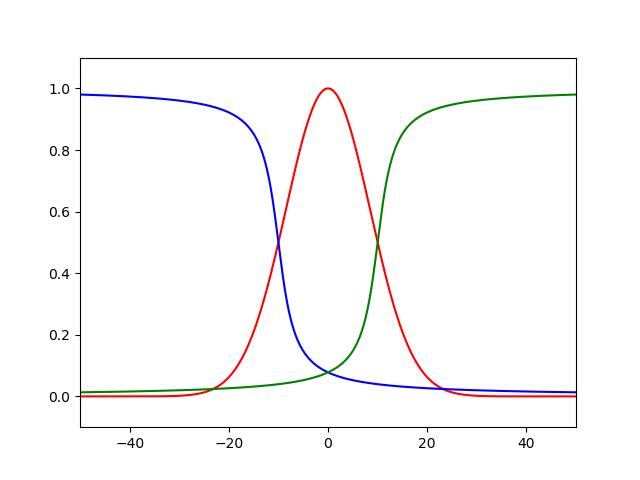
\includegraphics[width=0.6\textwidth]{obrazky-figures/fuzzysets.png}
\caption{Fuzzy sets used for fuzzification.\label{fig:fuzzysets}}
\end{center}
\end{figure}

Every edge gets assigned its fuzzy values for each of the classes. Now borders of artefacts need to be found.
Score of border $\xi[i]$ for the edge $x_i$ is evaluated using formula \ref{fig:artefactborder}.
\footnote{Operator $\land_P$ here means {\it product fuzzy T-norm}: $A \land_P B = f_A(x)\cdot f_B(x)$.}
The calculation is done for all the artefact combinations $ABC$ here, where $A$ is artefact of precedent $x_{i-1}$, $B$ for the
$x_i$ itself and $C$ for the follower $x_{i+1}$. $A,B,C \in \{F,S,B\}$.

% Artefact combination fuzzy formula.
\begin{equation}
\xi_{ABC}[i] = (\xi_{A}[i-1]) \land_P (\xi_{B}[i]) \land_P (\xi_{C}[i+1])
\label{fig:artefactborder}
\end{equation}

The combination indicating artefact border are put together as same as the rest. That is reached
using formula \ref{eq:edgemerger}.\footnote{Operator $\lor_{p\Sigma}$ here means
{\it probability sum fuzzy S-norm/T-conorm}: $A \lor_{p\Sigma} B = f_A(x) + f_B(x) - f_A(x)f_B(x)$.
Other variants could be considered too - maximum, Lukasiewicz, etc. } Border indicating
combinations are those, whose precedent and own combination differ, aka. {\it \{SF*, FS*, RF*, FR*, RS*, SR*\} }.
The rest, {\it \{FF*, SS*, RR*\}}, means no edge. The results are tresholded for $T = 0.5$.

% Artefact border fuzzy formula.
\begin{subequations}
\begin{equation}
f_{1}[i] = \bigvee\limits_{\xi \in \xi_1}{}_{p\Sigma} (\xi)
\end{equation}
\begin{equation}
f_{0}[i] = \bigvee\limits_{\xi \in \xi_0}{}_{p\Sigma} (\xi)
\end{equation}
\label{eq:edgemerger}
\end{subequations}


Newly created artefacts will be used to form feature vectors, filled with each one's characteristics.
Suggested metrics are variance and mean value of samples within artefact, scope of line, that 
can be counted using formula \ref{eq:artefactline}, etc.
$l_0$, $l_1$ are $y$ coordinates of first and last point of the line respectively,
\textbf{A} is a artefact samples vector. $k$ is the searched line scope,
$\Delta_{\textbf{A},k}$ is the difference score of artefact \textbf{A} and line with scope
$k$. It can also be used as a feature. This representation is to be seen in the figure \ref{fig:siglines}.

\begin{subequations}
\begin{equation}
l[i] = k\textbf{A}[i] + l_0
\end{equation}
\begin{equation}
k = \frac{l_1 - l_0}{|\textbf{A}|}
\end{equation}
\begin{equation}
\Delta _{\textbf{A},k} = \sum_{i \in \{1,...,|\textbf{A}|\}} (\textbf{A}[i]-l[i])^2
\end{equation}
\begin{equation}
l_0,l_1 = \text{argmin} ( \Delta_{\textbf{A},k} )
\end{equation}
\label{eq:artefactline}
\end{subequations}

\begin{figure}[h!]
\begin{center}
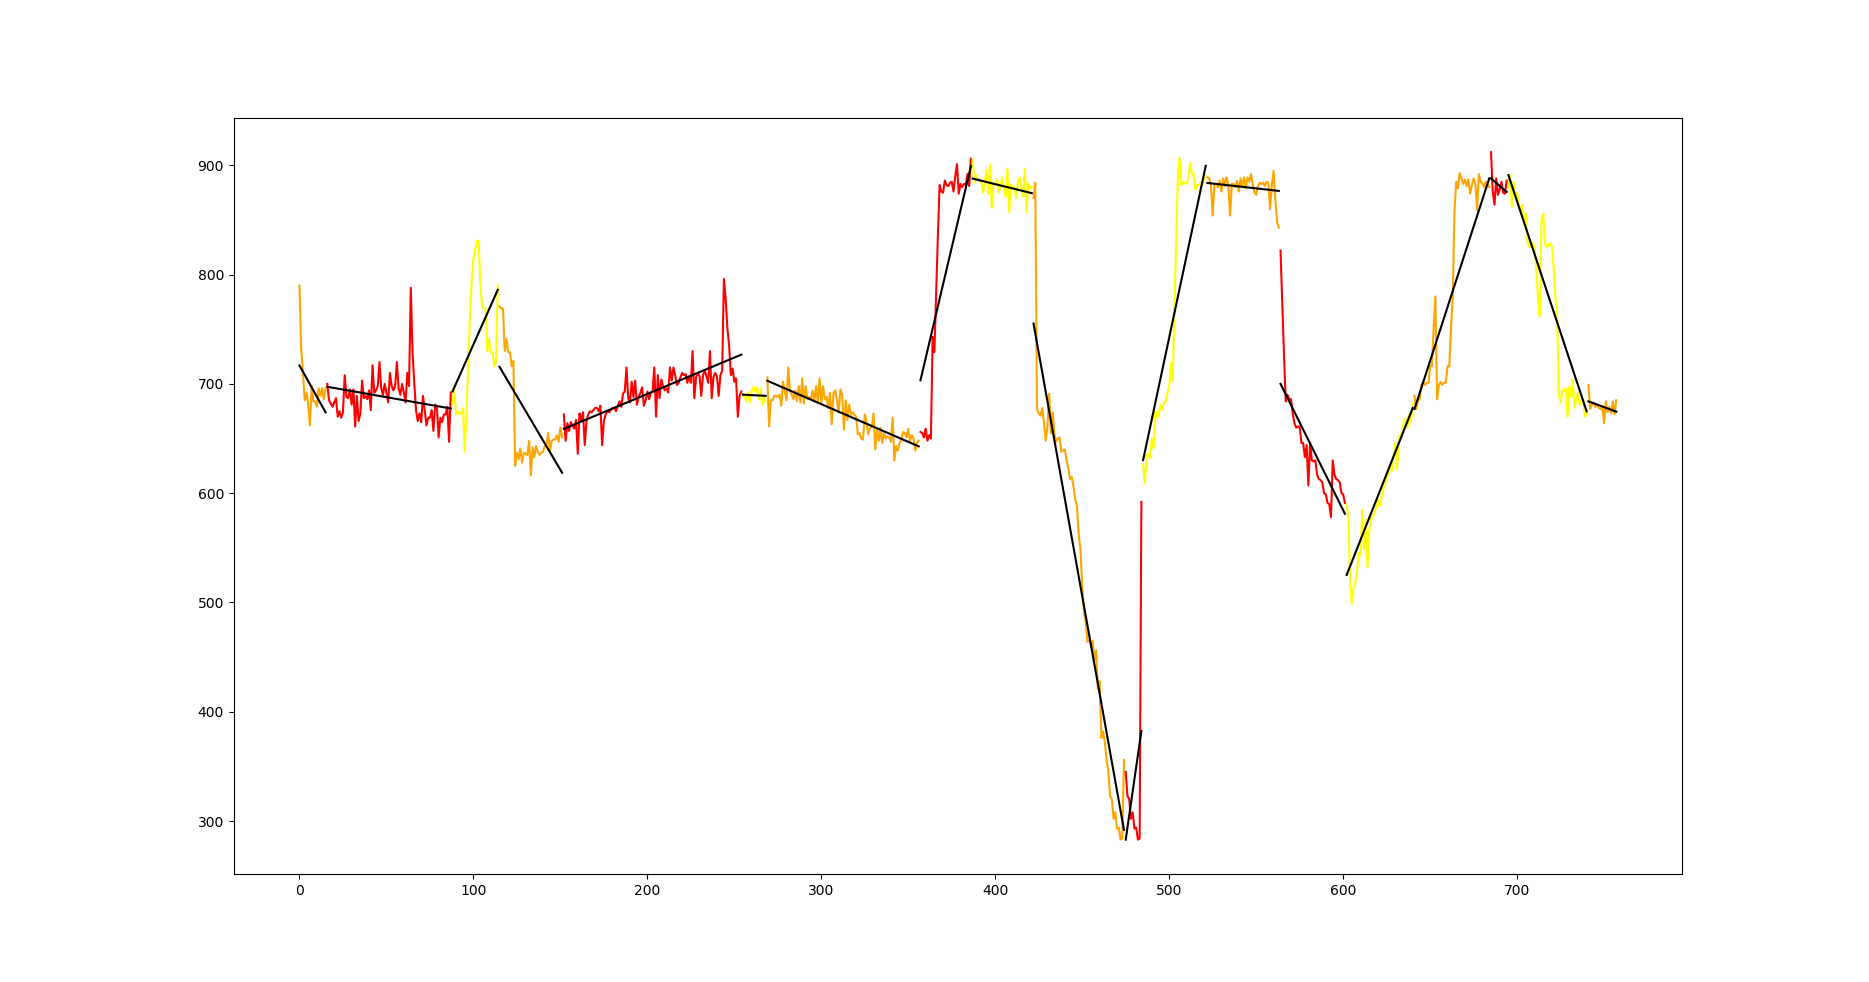
\includegraphics[width=0.85\textwidth]{obrazky-figures/signallines.png}
\caption{Representation of artefacts using line scope.\label{fig:siglines}}
\end{center}
\end{figure}

\subsection*{Classification}
Extracted feature vectors for every detected artefact will undergo classification procedure
consisting of multiple dichotomic classifiers, each evaluating single decision - whether
the movement is present or not, if the movement is towards center or aside, if the
movement is closer to sensor of far, and if possible, if the person is on the left side
or right.

The classification is process based on linear regression, searching for the best linear
separation of the training data using linear classifier \ref{eq:linearclassifier}, where 
$\overline{x}$ is an input, $\sigma(a)$ is activation function mapping
$\mathbb{R} \rightarrow \langle 0;1\rangle$ and $\overline{w}$,$w_0$ are searched parameters
of the classifier.


\begin{equation}
y(x) = \sigma (\overline{w}^T \overline{x} + w_0)
\label{eq:linearclassifier}
\end{equation}

The estimation of classifier's parameters $\overline{w}$,$w_0$ means maximizing the
posterior probabilities of each training data as same as solving the equation
\ref{eq:regressionEq}, in the logarithm domain \ref{eq:regressionLog}.

\begin{subequations}
\begin{equation}
p(t|\textbf{X}) = argmax \prod_{n \in C_1}y(\overline{x}_n) \prod_{n \in C_2} \{ 1 - y( \overline{x}_n ) \}
\label{eq:regressionEq}
\end{equation}
\begin{equation}
-\text{ln}( p(t|\textbf{X}) ) = - \sum_{n=1}^N \{ (t_n)\text{ln}(y_n) + (1-t_n)\text{ln}(1-y_n) \} = E(\overline{w})
\label{eq:regressionLog}
\end{equation}
\end{subequations}

The searched extrem of \ref{eq:regressionLog} means derivation \ref{eq:regressionGradient}
equal to $0$, solved numerically using \ref{eq:regressionGradientNumerical}.
$\eta \in (0;1\rangle$ is a converging parameter, the computation can be stopped either after
fixed step count or using minimal solution improvement $\varepsilon < | w^{(\tau + 1)} - w^{(\tau)} |$.

\begin{subequations}
\begin{equation}
\nabla E(\overline{w}) = \sum_{n=1}^N (y_n - t_n)x_n = 0
\label{eq:regressionGradient}
\end{equation}
\begin{equation}
w^{(\tau + 1)} = w^{(\tau)} - \eta \nabla E(\overline{w})
\label{eq:regressionGradientNumerical}
\end{equation}
\end{subequations}

Each of these scores are then fuzzified and put together, creating a resulting matrix.
The classifier's output is a 2D fuzzy value matrix, representing the space in from of the sensor.
It is inspired by the space representation by cellular automata, which carves it into small
homogenous segments. The fuzzy value at certain index expresses a presence of a person
at the position.

{\it Consider action characteristics (speed, direction, multiple people).}

Even though the space because of the construction of sensor has a shape of circular sector,
it can be easily represented by classical 2D matrix, as it is shown in the figure \ref{fig:circularsector}.

\begin{figure}[h!]
\begin{center}
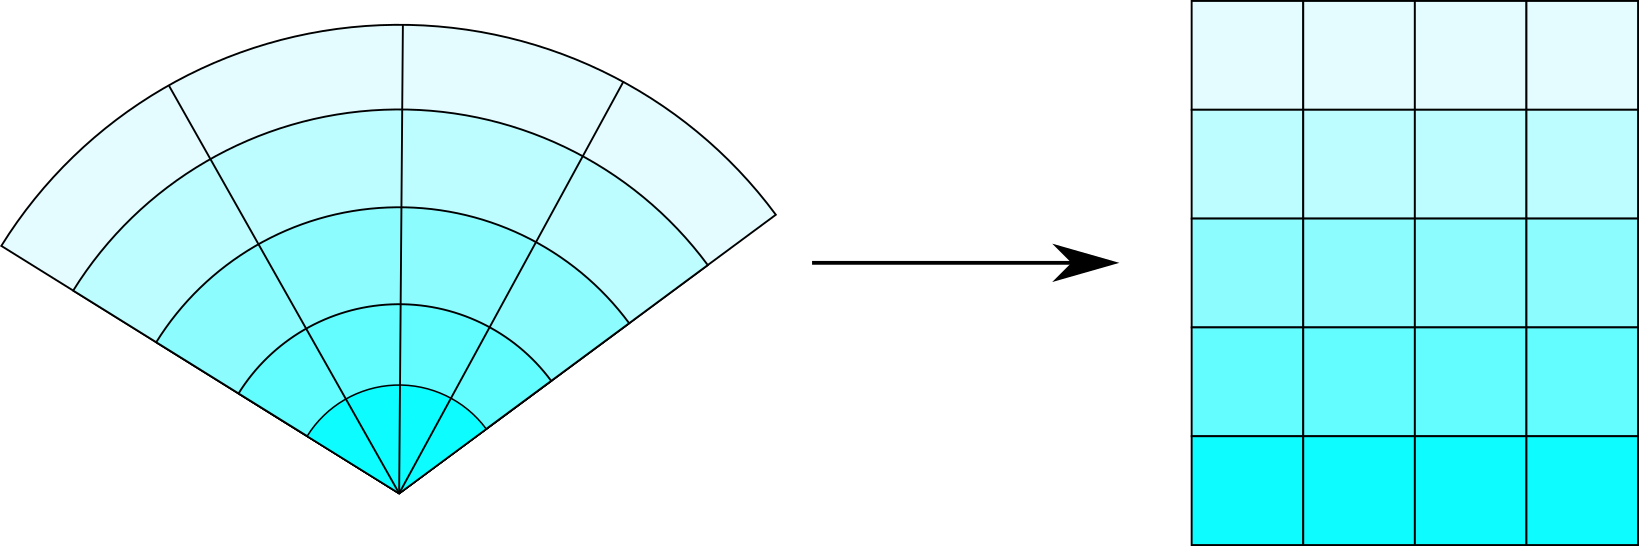
\includegraphics[width=0.5\textwidth]{obrazky-figures/circularsector_transformation.png}
\caption{Representation of circular sector.\label{fig:circularsector}}
\end{center}
\end{figure}


\subsection*{Fusion}
Using more sensors brings advantages: the measuring might be more precise since the person presence
classified by two independent sensors is not only more probable but the computed position
can get more accurate than when using only one sensor. The disadvantage is higher price and need
to know the mutual orientation and position of the sensors. 

%If more sensors are used it is necessary to merge their space segments matrixes in one,
%as shown in the figure \ref{fig:3pir_area}. To do so, a fuzzy logic mechanism
%{\it Takagi-Sugeno rules} can be used as described in \cite{InsightIntoFuzzyModelling}.
%The form of rules is [IF {\it antecendent} THEN {\it succendent}] as shown in the table
%\ref{table:takagisugeno}. During the calculation all the antecendentes are evaluated
%and the most relevant leads to application of corresponding succendent to the output.

%\begin{figure}[h!]
%\begin{center}
%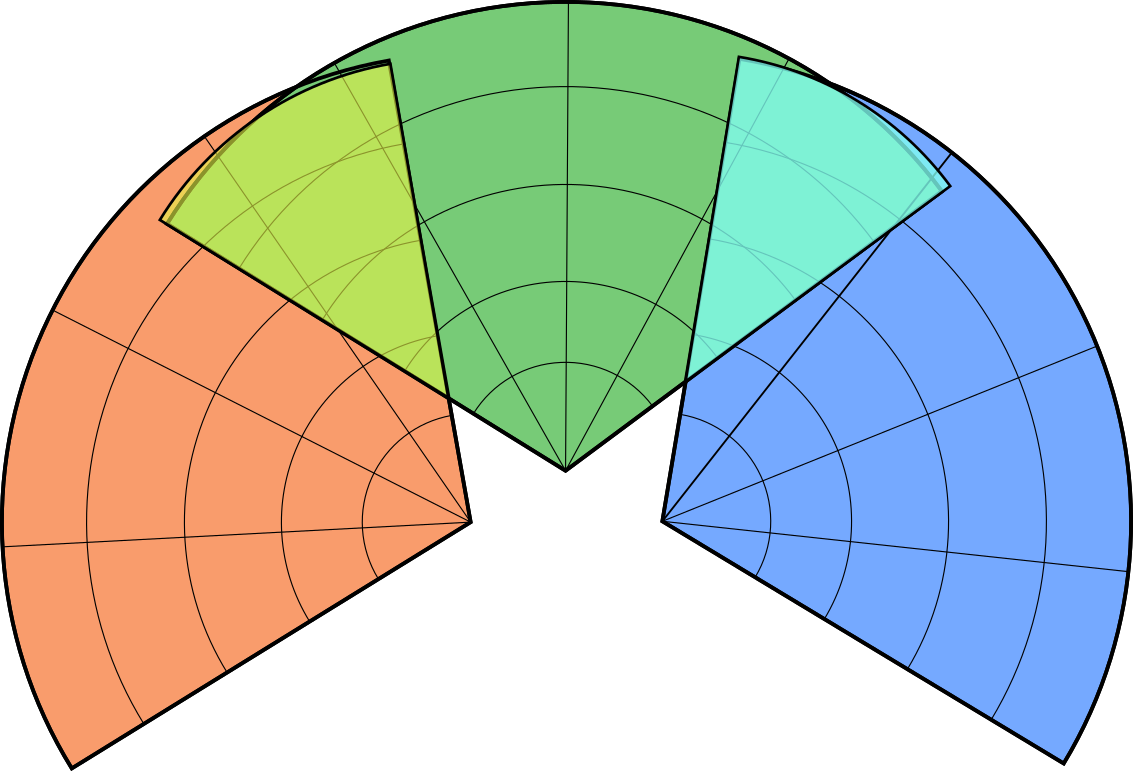
\includegraphics[width=0.5\textwidth]{obrazky-figures/3pir_area.png}
%\caption{Fusion of detection areas.\label{fig:3pir_area}}
%\end{center}
%\end{figure}

%\begin{table}[h!]
%\begin{center}
%\begin{tabular}{|c|c|c|} \hline
%\textbf{Rule}   & \textbf{Antecendent}                                & \textbf{Succendent}                             \\ \hline
%$R_1$           & $X_1$ is $A_{11}$ and \dots and $X_n$ is $A_{1n}$   & $Y = b_{10} + b_{11}X_1 + \dots + b_{1n}X_n$    \\ \hline
%$R_2$           & $X_1$ is $A_{21}$ and \dots and $X_n$ is $A_{2n}$   & $Y = b_{20} + b_{21}X_1 + \dots + b_{2n}X_n$    \\ \hline
%\multicolumn{3}{|c|}{\dots}                                                                                             \\ \hline
%$R_m$           & $X_1$ is $A_{m1}$ and \dots and $X_n$ is $A_{mn}$   & $Y = b_{m0} + b_{m1}X_1 + \dots + b_{mn}X_n$    \\ \hline
%\end{tabular}
%\caption{Takagi-Sugeno rules. $X$ is input, $A$ is a matrix of fuzzy numbers, $b$ is a matrix of fuzzy coefficients.\label{table:takagisugeno} \cite{InsightIntoFuzzyModelling}}
%\end{center}
%\end{table}

%The designed fusion fuzzy system is to be seen in the table \ref{table:fuzzyfusion}. To be able to merge
%the space segments, overlap must be known and then vector $X$ is created, containing pairs of values
%from each vector ($X[i]_L$ and $X[i]_R$). Each of these pairs is input to the fusion algorithm, which
%merges it to one fuzzy number result. 

%$C_{L}$ and $C_{R}$ are 2D matrixes of coefficients with indexing $[i,j]$, where $i,j \in \{0,L,M,H\}$.
%The fuzzy sets LOW, MEDIUM and HIGH of $X$ composes a basic evaluative trichotomy extended for unknown state OUT.
%The optimal values of coefficients and the fuzzy sets parameters have to be found experimentally. 

%\begin{table}[h!]
%\begin{center}
%\begin{tabular}{|c|c c|rcl|} \hline
%\textbf{Rule}   & \textbf{$X_L$}  & \textbf{$X_R$}  & \multicolumn{3}{|c|}{\textbf{Y}}  \\ \hline
%$R_1$           & OUT             & OUT             & $C_{L}[0,0]    $&+&$ C_{R}[0,0]   $   \\ \hline
%$R_2$           & OUT             & LOW             & $C_{L}[0,L]    $&+&$ C_{R}[L,0]X_R$   \\ \hline
%$R_3$           & OUT             & MEDIUM          & $C_{L}[0,M]    $&+&$ C_{R}[M,0]X_R$   \\ \hline
%$R_4$           & OUT             & HIGH            & $C_{L}[0,H]    $&+&$ C_{R}[H,0]X_R$   \\ \hline
%$R_5$           & LOW             & OUT             & $C_{L}[L,0]X_L $&+&$ C_{R}[0,L]   $   \\ \hline
%$R_6$           & LOW             & LOW             & $C_{L}[L,L]X_L $&+&$ C_{R}[L,L]X_R$   \\ \hline
%$R_7$           & LOW             & MEDIUM          & $C_{L}[L,M]X_L $&+&$ C_{R}[M,L]X_R$   \\ \hline
%$R_8$           & LOW             & HIGH            & $C_{L}[L,H]X_L $&+&$ C_{R}[H,L]X_R$   \\ \hline
%$R_9$           & MEDIUM          & OUT             & $C_{L}[M,0]X_L $&+&$ C_{R}[0,M]$      \\ \hline
%$R_{10}$        & MEDIUM          & LOW             & $C_{L}[M,L]X_L $&+&$ C_{R}[L,M]X_R$   \\ \hline
%$R_{11}$        & MEDIUM          & MEDIUM          & $C_{L}[M,M]X_L $&+&$ C_{R}[M,M]X_R$   \\ \hline
%$R_{12}$        & MEDIUM          & HIGH            & $C_{L}[M,H]X_L $&+&$ C_{R}[H,M]X_R$   \\ \hline
%$R_{13}$        & HIGH            & OUT             & $C_{L}[H,0]X_L $&+&$ C_{R}[0,H]   $   \\ \hline
%$R_{14}$        & HIGH            & LOW             & $C_{L}[H,L]X_L $&+&$ C_{R}[L,H]X_R$   \\ \hline
%$R_{15}$        & HIGH            & MEDIUM          & $C_{L}[H,M]X_L $&+&$ C_{R}[M,H]X_R$   \\ \hline
%$R_{16}$        & HIGH            & HIGH            & $C_{L}[H,H]X_L $&+&$ C_{R}[H,H]X_R$   \\ \hline
%\end{tabular}
%\caption{Design fuzzy system to fuseTakagi-Sugeno rules. $X$ is input, $A$ is a matrix of fuzzy numbers, $b$ is a matrix of fuzzy coefficients.\label{table:fuzzyfusion} \cite{InsightIntoFuzzyModelling}}
%\end{center}
%\end{table}

%For three sectors as in the figure \ref{fig:3pir_area} the situation is analogous. The table also depends
%on whether the areas of the side sensors overlap or not. Or they can be merged successively.

\subsection*{Defuzzification}

To get the results in a form of coordinate(s) of classified objects a cluster analysis is done. It calculates
a clusters of high membership values, for optimalization $\alpha$-cut on a certain level or tresholded
matrix can be used. Algorithm PAM (Partitioning Around Medoids is used), similar to k-means, where item called
medoid is used to represent the cluster instead of mean.

\begin{equation}
\mathit{PAM}(k, data) = argmin \left( \sum_{i=1}^{k} \sum_{j=1}^{k} ||data_{i} data_{j}||  \right)
\end{equation}

\begin{lstlisting}[style=python]
def PAM(k,data):
  # pick medoids
  medoids = [].generate(k,data.random())
  # compute dissimilarity matrix
  dm = DissimilarityMatrix(data,calculateDistance)
  # create clusters
  changed = True
  while changed:
    changed = False
    clusters = []
    for medoid_idx,medoid in medoids.enum():
      cluster = []
      for d in data:
        # add to cluster with closest distance to its medoid
        if dm[d,medoid] == dm[d,medoids].min():
          cluster.append(d)
      # set new center (SWAP phase)
      cluster.append(medoid)
      if medoid is not cluster.center():
        medoids[medoid_idx] = cluster.center()
        changed = True
      clusters.append(cluster)
  return clusters
\end{lstlisting}

\begin{lstlisting}[style=python]
function elbow(data):
  # try all k
  best = inf
  for k in <1,K_MAX>:
    clusters = PAM(data, k)
    # take minimal
    if WCSS(clusters) < best:
      best = clusters
  return best
\end{lstlisting}

To estimate the $k$, elbow method can be used: calculating k-means for different k values and taking the one with
minimal within-cluster sum of square (WCSS).\cite{ClusterAnalysis} \cite{VagueNatureInformation}

\begin{equation}
\mathit{WCSS} = \sum_{i=1}^{k} \sum_{x \in S_i} ||x - \mu_i||^2
\end{equation}

Very important is computing a distance of two segments. Since the original circular sector segmentation
is not homogenous, the distances varies with each distance. It can be calculated though using
cosine law. $P = (d, \alpha)$ is a segment given by polar coordinates, $d$ is distance and $\alpha$ is
azimuth.

\begin{equation}
|P_{1} P_{2}| = \sqrt{(d_{1})^{2} + (d_{2})^{2} - 2d_{1}d_{2}(\alpha_1 - \alpha_2)}
\end{equation}




\chapter{Data}

\begin{figure}[h!]
\begin{center}
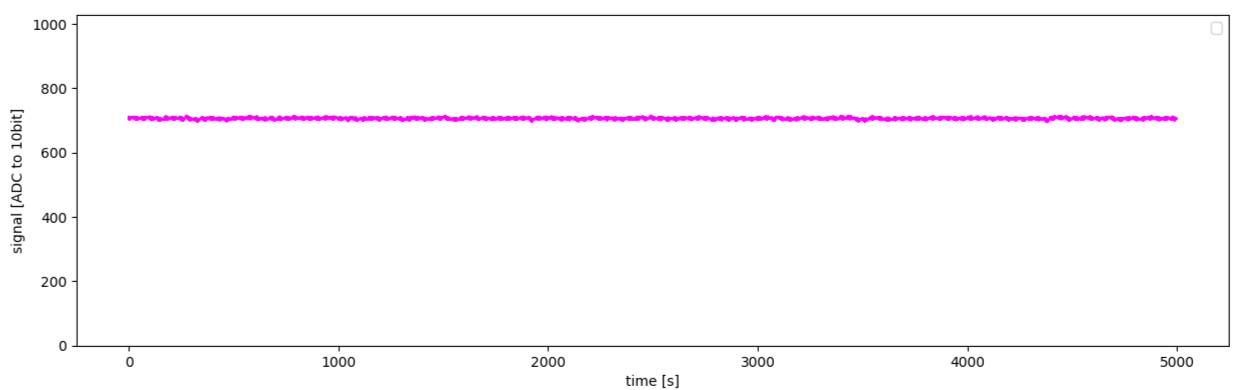
\includegraphics[width=0.85\textwidth]{obrazky-figures/signal_calm.png}
\caption{Signal of zero movement.\label{fig:signalcalm}}
\end{center}
\end{figure}

\begin{figure}[h!]
\begin{center}
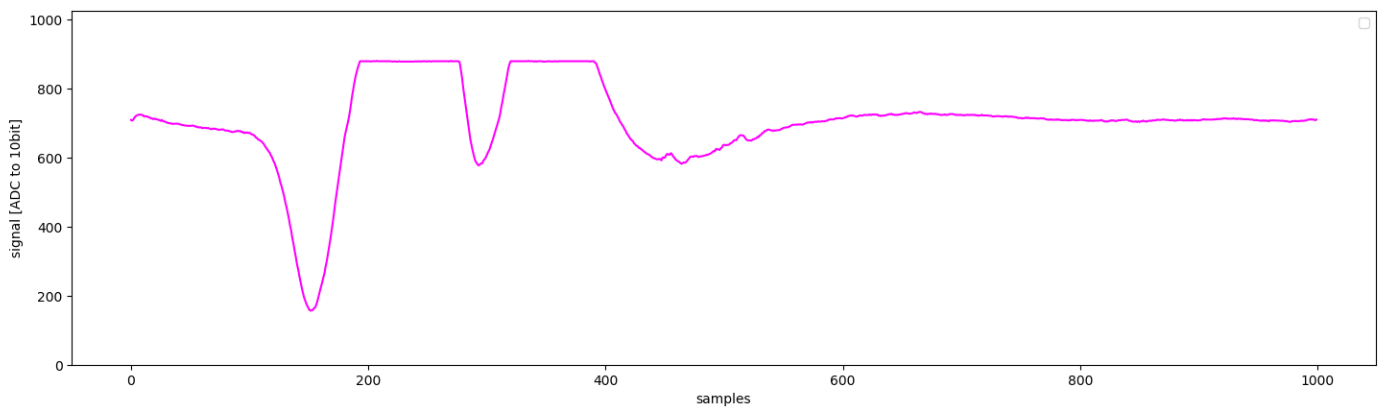
\includegraphics[width=0.85\textwidth]{obrazky-figures/signal_walk.png}
\caption{Signal of person walking around.\label{fig:signalwalk}}
\end{center}
\end{figure}

A output of a sensor as you can see in the figures \ref{fig:signalcalm} and \ref{fig:signalwalk}
is very discriminative -- with a bare eye a movement from no movement is distinguishable.
A detection of presence used in light sensors can be implemented with tresholding, this attitude is
not very suitable for classification of anything else except the presence itself.

In a calm state the sensor sends a constant signal\footnote{Constant signal in the terms
of electricity, slightly polluted with a background noise etc.}. Movement in the sensed area causes
abrupt changes of output. When the object either leaves the area, or stays completely calm, the signal
changes are getting slower and after a little while the output voltage gets in the calm state again.

Therefore, the nature of the signal does not seem to need a complicated method to perform a classification on it.
{\it Fourier transformation} and {\it wavelet transformation} were considered for feature
extraction. The abrupt changes in the signal could be problem for FT, because it can not represent
it efficiently\cite{SinglePIR}, % youtube video
but unlike sinusoids, the wavelets exist for a finite duration and they are suitable for representing
abrupt changes.

The wavelet transformation is defined as a function F(s,k). Parameters s,k are scale and shift, changing
them in predefined unit and interval creates a matrix, as you can see in the figure \ref{fig:walk03}.

\begin{equation}
F(s,k) = \sum_{n=1}^{N} x[n] \Psi_{(s,k)}^{*}[n]
\end{equation}

Firstly The data were offline analysed using {\it Matlab}, which has implemented wavelet transformation.
The Matlab is not used because it is proprietary software and the program would be dependent on it.
During the analysis it was found, that the data are very well separable using continuous wavelet tranformation.

\begin{figure}[h!]
\begin{lstlisting}[style=matlab]
data = csvread('walk02.csv');
wscalogram('image', cwt(data));
\end{lstlisting}
\caption{Matlab code performing cwt.\label{list:cwtmatlab}}
\end{figure}

\begin{figure}[h!]
\begin{center}
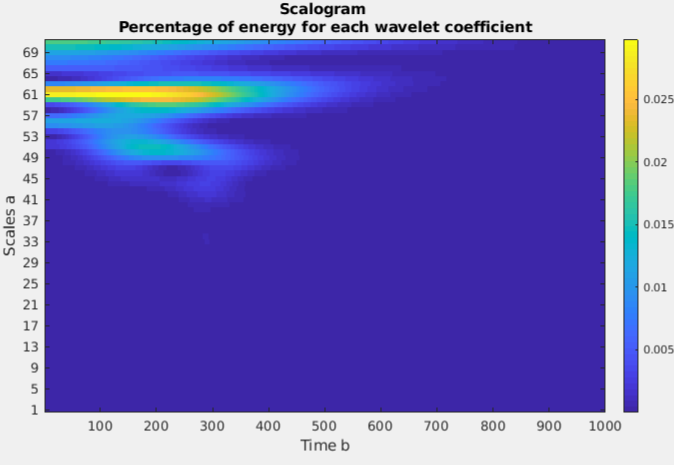
\includegraphics[width=0.6\textwidth]{obrazky-figures/walk03.png}
\caption{Matlab {\it cwt()} output of {\it walk03.csv}.\label{fig:walk03}}
\end{center}
\end{figure}


{\it Origin of data, description, training.}

The lab results are shown in the appendix \ref{appendix:PIRSignal}.




\chapter{Implementation}

\section{Sensor device}

The sensor device consists of PIR sensor and programmed MCU that samples analog signal from
sensor and writes in chunks called segments it via WiFi to local multicast group.

Nowadays most of the PIR sensors sold have only a binary {\it switching} output.
When signal reaches a set treshold output is set to logic "1" for a unit of time.
This mechanism is suitable for a light sensor or door sonsor, completely useless
for the needs of this project though.

The only found sensor that offers an analog output was {\it PIR STD} by
{\it B+B Sensors}.

\subsection*{PIR STD}
{\it PIR STD} is a product of {\it B+B Sensors}. It is the only found passive infrared
sensor, that has except of the switching binary ouput also analog output. Except of
operating voltage $V_{cc}$ and ground $GND$ pins, it also has reference voltage input,
which needs to be connected to $\frac{V_{cc}}{2} V$. The optical resistance pins can
be also used for additional classification, fusion with the infrared signal classification
results and making the final result more accurate.

Pin layout table from the sensor operational manual is shown in the table \ref{fig:pirstdpin}.

\begin{table}[h!]
\begin{center}
\begin{tabular}{|c c | c | c |} \hline
\textbf{Pin} & \textbf{Code} & \textbf{Type} & \textbf{Description} \\ \hline
1 & ANA & O & Analog output \\ \hline
2 & REF & I & Reference voltage \\ \hline
3 & GND & O & Ground \\ \hline
4 & OUT & O & Binary (switching) output \\ \hline
5 & GND & O & Ground \\ \hline
6 & VCC & I & Operating voltage \\ \hline
7 & LDR & O & Optical resistance \\ \hline
8 & LDR & I & Optical resistance \\ \hline
\end{tabular}
\end{center}
\caption{Pin layout of PIR STD.\cite{PIROperationalManual}\label{fig:pirstdpin}}
\end{table}

The {\it PIR STD} scheme shown in the figure \ref{fig:pirstdscheme} processes the signal
in three stages going from left to right. The first two filter and amplify the signal
resulting with analog output. The third generates binary output from analog.

\begin{figure}[h!]
\begin{center}
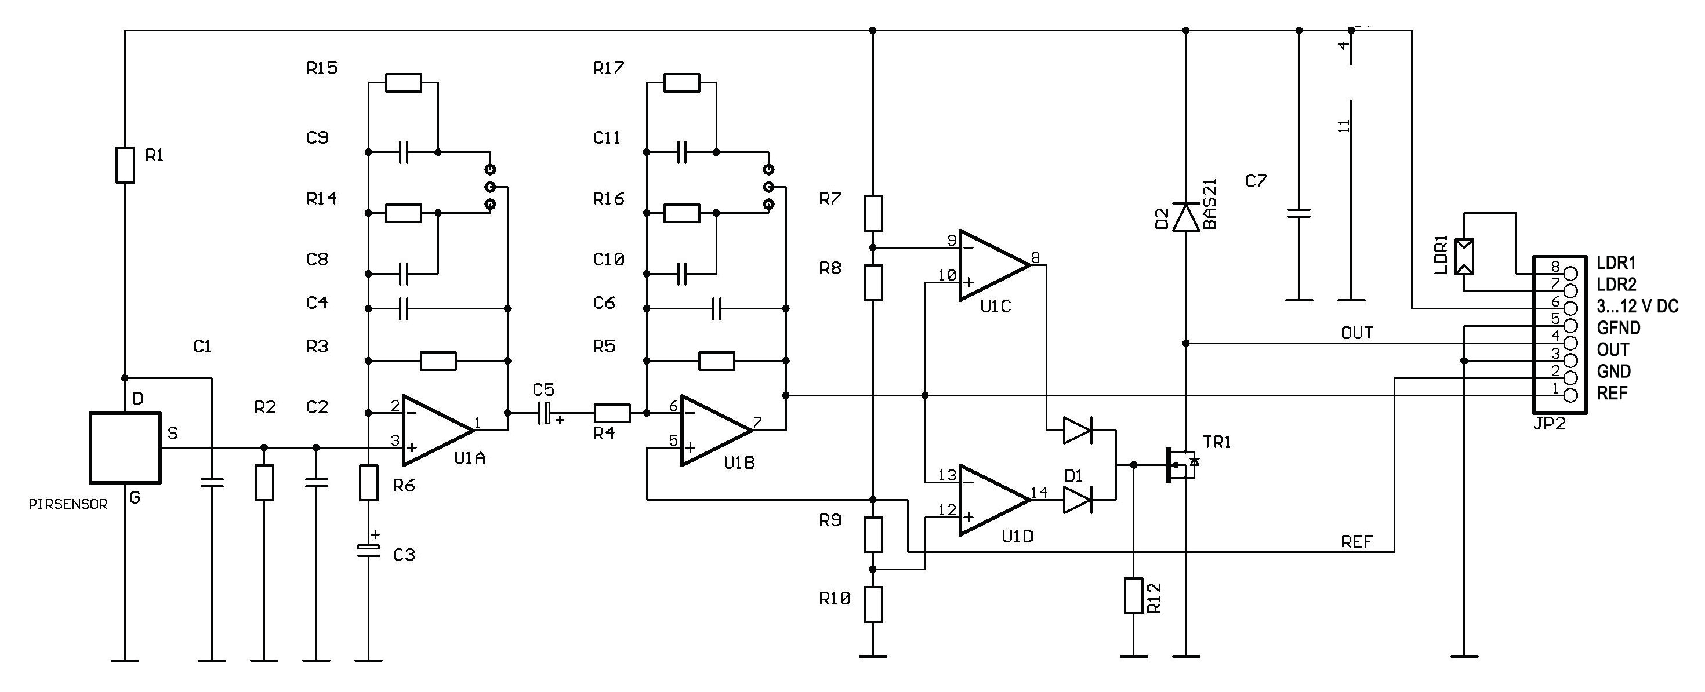
\includegraphics[width=0.75\textwidth]{obrazky-figures/pirstd.png}
\caption{Scheme of PIR STD.\cite{PIROperationalManual}\label{fig:pirstdscheme}}
\end{center}
\end{figure}

\paragraph{I. stage}
The first one starts at S of the PIR sensor, following with noise/lowpass filter consisting
of the amplifier $U1A$ and the feedback components $R3$, $C4$, $C8$, $R14$, $C9$, $R14$.
There is also highpass filter done by $R6$ and $C3$. The output of this stage is a signal
with frequency between $f_{L1}$ and $f_{H1}$ amplified $A_{U1A}$ times.

\begin{subequations}
\begin{equation}
f_{H1} = \frac{1}{2 \pi R_{3,14} C_{4,8}}
\end{equation}

\begin{equation}
f_{H1}^{'} = \frac{1}{2 \pi R_{3,15} C_{4,9}}
\end{equation}
\end{subequations}

The choice of resistor $R_{3,14} / R_{3,15}$ and capacitator $C_{4,8} / C_{4,9}$
is done by connected switch. The value of resistance and capacitance of the
components can be counted with formula for parallel connection.

\begin{equation}
R_{A,B}^{p} = \frac{1}{R_A} + \frac{1}{R_B}
\end{equation}

\begin{equation}
C_{A,B}^{p} = C_A + C_B
\end{equation}

The same for the resistors $R_{5,16}$ and $R_{5,17}$ and capacitators $C_{6,10}$ and $C_{6,11}$.

\begin{equation}
f_{L1} = \frac{1}{2 \pi R_6 C_3}
\end{equation}

\begin{subequations}
\begin{equation}
A_{U1A} = 1 + \frac{R_{3,14}}{R_2}
\end{equation}
\begin{equation}
A_{U1A} = 1 + \frac{R_{3,15}}{R_2}
\end{equation}
\end{subequations}

\paragraph{II. stage}
The second processing stage focuses on amplification. It also includes lowpass filtering done
by $C5$ and $R4$ and highpass filter performed by the feedback of amplifier $U1B$. The greater
amplification is also made by the divider bridge ($R8$, $R9$, $R10$, $R11$) connected to the
positive input. The output of frequency between $max(f_{L1}, f_{L2})$ and $min(f_{H1}, f_{H2})$
amplified $A_{U1A} \cdot A_{U1B}$ times is an analog output connected to the pin 1.

\begin{equation}
f_{H2} = \frac{1}{2 \pi R_5 C_6}
\end{equation}

\begin{equation}
f_{L2} = \frac{1}{2 \pi R_4 C_5}
\end{equation}

\begin{equation}
A_{U1B} = -\frac{R_5}{R_4}
\end{equation}

\paragraph{III. stage}
The third phase performs top-bottom tresholding generating binary output
used in simple industrial application. It is not used in the project.\cite{PIRSchemeDescription}


\subsection*{Connecting the sensor}
PIR sensor is connected to the MCU. Except for source, ground and output which are connected directly,
{\it PIR STD} has also reference voltage input, that should be approximately $\frac{V_cc}{2}~V$.
To ensure that a voltage divider is used with two resistors of the same resistance $R_X$.
During the testing $100~k\Omega$ resistors were used. The circuit is shown in the figure \ref{fig:PIRcircuit}.

\begin{figure}[h!]
\begin{center}
\begin{circuitikz}
\ctikzset{bipoles/generic/height=0.2}
\ctikzset { label/align = straight }
\draw %(2,0)

  %to[V=$V_{Th}$] (0,2)
  %to[R=$R_{Th}$] (2.5,2)
  %to[short,i=$I$, -o] (4,2)
  %to[short] (4.5,2)
  % ref
  (0,2) to[short, l={\tiny $REF$}, o-]
  (1,2) to[short]
  (2,2) to[R={\tiny $R_{X}$}]
  (4,2) to[R={\tiny $R_{X}$}]
  (6,2) to[short,-*] (6,0.5)
  
  (4,2) to[short,*-*] (4,1.5)
  % vcc
  (0,1.5) to[short, l={\tiny $VCC$}, o-]
  (1,1.5) to[short]
  (7,1.5) to[short, l={\tiny $5~V$}, -o] (8,1.5)
  % signal
  (0,1) to[short, l={\tiny $ANA$}, o-] 
  (1,1) to[short]
  (7,1) to[short, l={\tiny $A1$}, -o] (8,1)
  % gnd
  (0,0.5) to[short, l={\tiny $GND$}, o-]
  (1,0.5) to[short]
  (7,0.5) to[short, l={\tiny $GND$}, -o] (8,0.5)

;
\node[draw,minimum width=2.5cm,minimum height=2.5cm,anchor=south east] at (0,0){PIR};
\node[draw,minimum width=2.5cm,minimum height=2.5cm,anchor=south west] at (8,0){MCU};
\end{circuitikz}
\caption{Connection of PIR and MCU.\label{fig:PIRcircuit}}
\end{center}
\end{figure}


\subsection*{Sampling}
The module is programmed to read signal in sampling frequency and send the data to server.

\paragraph{AD conversion}
The projection of voltage to a value is done by the built-in functionality, accessible by
standard library function \texttt{analogRead()}. The sets of analog values $A$ and digital values $D$
according to documentation of the function\cite{ArduinoAnalogRead} and the sensor\cite{PIROperationalManual}
and the morphism $c$ are shown in the formula \ref{eq:ad_projection}.

\begin{subequations}
\begin{equation}
A = <0;V_{cc}>
\end{equation}
\begin{equation}
D = {0, 1, ..., 1023}
\end{equation}
\begin{equation}
c: A \rightarrow D = x_A \rightarrow \frac{1023x_A}{V_{cc}}, x_A \in D
\end{equation}
\end{subequations}

\paragraph{Sampling frequency}
The usable sampling frequency can be estimated: the fresnel lens of {\it PIR STD} splits the
area into $10^{\circ}$ circular sectors. Object moving around the sensor in the distance $0.5~m$
with speed $15~km.h^{-1} = 4.1667~m.s^{-1}$ (very fast run) passes the central circular sector in

\begin{equation}
t = \frac{s}{v} = \frac{0.5*tg(10^{\circ})}{4.1667} = 0.02116~s
\end{equation}

This means the frequency of the movement through the circular sectors is

\begin{equation}
f = \frac{1}{t} = \frac{1}{0.02116} = 47.259~Hz
\end{equation}

According to Shannon theorem\cite{DigitalSignalProcessing}, the sampling frequency must be at least twice as big as the
maximal frequency in the signal, which leads to

\begin{equation}
Fs \geq 2*47.259 = 94.518 
\end{equation}

Rounding up gives us minimal sampling frequency $100~Hz$, or sampling period $10~ms$.
resulting with $2B$ sample in throughput $\mu$

\begin{equation}
\mu = F_s * |\text{sample}| * 8\frac{bit}{byte} = 100 * 2 * 8 = 1.6~kbps
\end{equation}


\subsection*{MCU Program}
The MCU is programmed to sample data with fixed sampling frequency and form the sequential
segments out of it. A $N$-sized segment is then sent away using ESP8266 present at the module.
A multicast technology is used, enabling multiple servers to work over the data concurrently
and also ease of initialization of communication, where the channel is predefined, so
no mutual IP address is needed. The sending frequency can be derived from sampling frequency $F_s$
with formula \ref{eq:sendfrequency}.

\begin{equation}
F_{send} = \frac{F_s}{N}
\label{eq:sendfrequency}
\end{equation}

MCU runs a HTTP server, enabling the MCU to be configured remotely. It is possible to set
sampling frequency or period with the altering other correspondingly as same as sending period,
frequency, or segment size with a maximal segment size \textbf{here will be MAXSEGMENTSIZE}.
The REST API also enables to set the multicast channel, both address and port, turning
debugging informations on/off to serial line.

The complete REST API description is to be seen in the appendix \ref{appendix:mcu_restapi}.




\section{Classification server}
{\it Monitor} is the classification server, that collects data from the sensors and performs
classification algorithms described in \ref{section:classification} with it. {\it Finish}

\subsection*{Data sources}
Monitor enables reading data from serial port, multicast channel and replaying saved data from file.
This feature is done using class \texttt{Reader} from the module \texttt{comm} and inherited classes
in modules \texttt{comm\_serial}, \texttt{comm\_mcast}, \texttt{comm\_replay}.

Class Reader corresponds with the design pattern Singleton, holding one single instance for each
serial port, multicast channel and file to avoid opening multiple handles and potential data race.

Instantiation of the object is done in the first demand for it in the call of static method \texttt{getReader()}.
Each object then possess separate reading thread, that ensures updating of the data. Getting the last
received segment is through method \texttt{getSegment()}, a thread lock is used. The whole design is shown
in the figure \ref{fig:class_src}.

\begin{figure}[h!]
\begin{center}
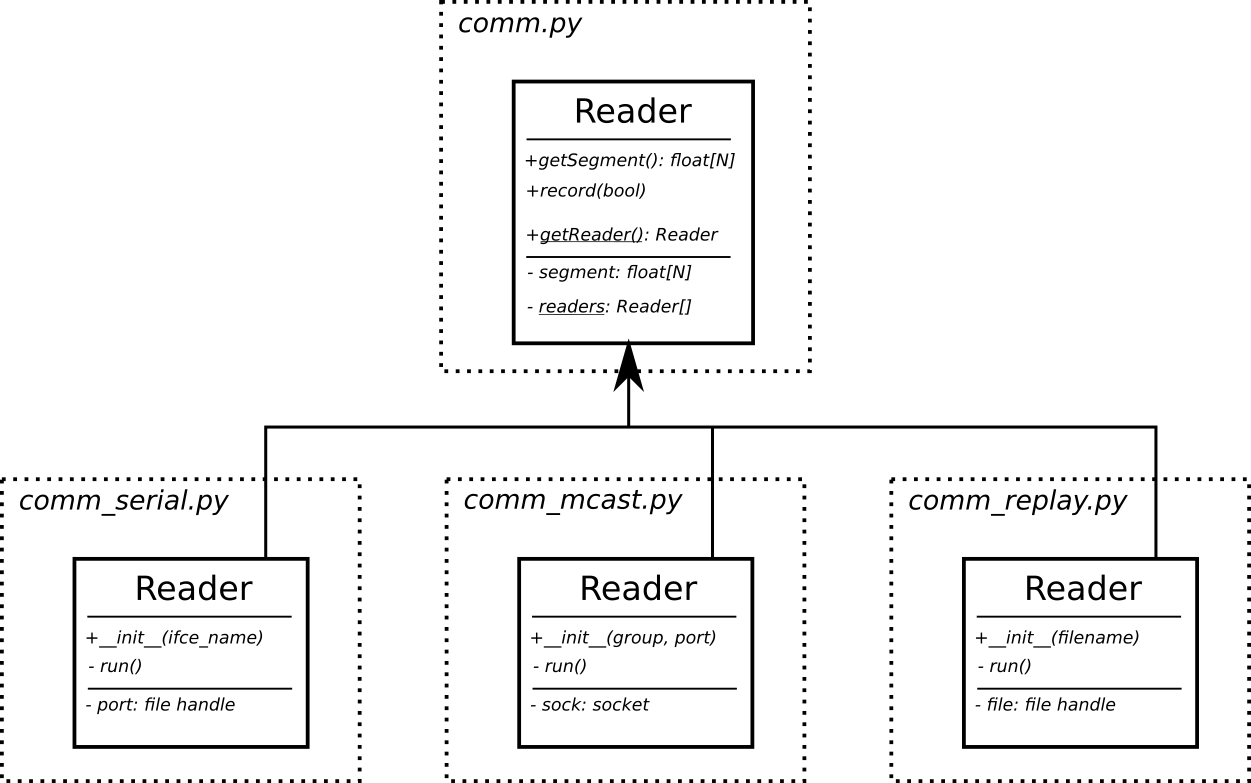
\includegraphics[width=0.8\textwidth]{obrazky-figures/class_src.png}
\caption{UML diagram of Reader classes. \label{fig:class_src}}
\end{center}
\end{figure}

{\it ...}

\subsection*{Classification}
{\it Implementation of linear regression.}







%\section{Collector} 
%{\it Collector} is a program, as the name says, that collects data from sensors and implements
%the whole described algorithm. Classified objects are then sent to a {\it visualizer}.

%\subsection*{Communication}
%The communication of the sensor module and the client app is designed as a client-server. The results
%from the classification performed by server are sent to the client which shows it to user.

%As the technology for the channel a LAN multicast stream is used at 224.0.0.128:12345.
%The main advantage in comparison to unicast is a support of multiple clients.

%\section{Visualizer}
%Client app called {\it Visualizer} is written in {\it Python3} and graphical library {\it Tkinter}.
%This choice was made with portability of the program taken into consideration.
%The design of user interface is described in chapter \ref{Label:UI}.




\chapter{Experiments}
Unit tests were created to verify the program components. It uses {\it Boost.Test},
framework for creating unit tests which is part of {\it C++ Boost} library set.
The testing program placed in folder {\it collector/tests/} is linked with
{\it collector} transformed in static library.

{\it
Metodika a vysledky. Muze zahrnovat i matematicke dukazu, postupy...

Interpretace vysledku a moznosti nasazeni v praxi.

HW narocnost -- CPU, pamet, chovani pri paralelizaci apod.
}




\chapter{User Interface}
\label{Label:UI}

{\it Description of visualizer}

\begin{figure}[h!]
\begin{center}
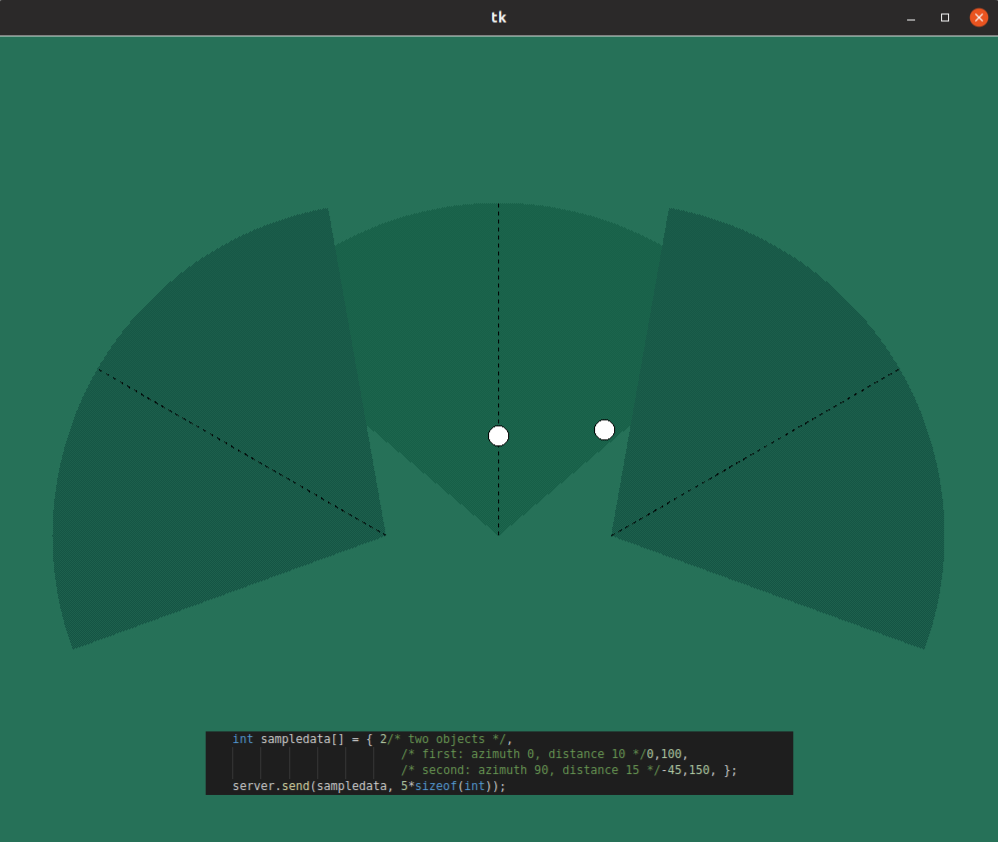
\includegraphics[width=0.6\textwidth]{obrazky-figures/visualizer.png}
\caption{Visualizer prototype with sample data. {\it Will be replaced.} \label{fig:visualizer}}
\end{center}
\end{figure}






\chapter{Conclusion}
Shrnuti zameru prace. Zhodnoceni splneni (i formalnich bodu).

Zhodnoceni z pohledu dalsiho vyvoje. Co se nestihlo (a dalo by se jeste).

Bez odkazu do textu / literatury. Zadne nove poznatky, cisla a grafy.

Pekny postreh k praci (co jsem se naucil).

Vyhled do budoucna, rozdeleni na casti.

20 stranek SEP, 40 bakalarka.




%===============================================================================

  
  % Kompilace po částech (viz výše, nutno odkomentovat)
  % Compilation piecewise (see above, it is necessary to uncomment it)
  %\subfile{projekt-01-uvod-introduction}
  % ...
  %\subfile{chapters/projekt-05-conclusion}


  % Pouzita literatura / Bibliography
  % ----------------------------------------------
\ifslovak
  \makeatletter
  \def\@openbib@code{\addcontentsline{toc}{chapter}{Literatúra}}
  \makeatother
  \bibliographystyle{bib-styles/slovakiso}
\else
  \ifczech
    \makeatletter
    \def\@openbib@code{\addcontentsline{toc}{chapter}{Literatura}}
    \makeatother
    \bibliographystyle{bib-styles/czechiso}
  \else 
    \makeatletter
    \def\@openbib@code{\addcontentsline{toc}{chapter}{Bibliography}}
    \makeatother
    \bibliographystyle{bib-styles/englishiso}
  %  \bibliographystyle{alpha}
  \fi
\fi
  \begin{flushleft}
  \bibliography{xbenes49-20-literatura-bibliography}
  \end{flushleft}

  % vynechani stranky v oboustrannem rezimu
  % Skip the page in the two-sided mode
  \iftwoside
    \cleardoublepage
  \fi

  % Prilohy / Appendices
  % ---------------------------------------------
  \appendix
\ifczech
  \renewcommand{\appendixpagename}{Přílohy}
  \renewcommand{\appendixtocname}{Přílohy}
  \renewcommand{\appendixname}{Příloha}
\fi
\ifslovak
  \renewcommand{\appendixpagename}{Prílohy}
  \renewcommand{\appendixtocname}{Prílohy}
  \renewcommand{\appendixname}{Príloha}
\fi
%  \appendixpage

% vynechani stranky v oboustrannem rezimu
% Skip the page in the two-sided mode
%\iftwoside
%  \cleardoublepage
%\fi
  
\ifslovak
%  \section*{Zoznam príloh}
%  \addcontentsline{toc}{section}{Zoznam príloh}
\else
  \ifczech
%    \section*{Seznam příloh}
%    \addcontentsline{toc}{section}{Seznam příloh}
  \else
%    \section*{List of Appendices}
%    \addcontentsline{toc}{section}{List of Appendices}
  \fi
\fi
  \startcontents[chapters]
  \setlength{\parskip}{0pt}
  % seznam příloh / list of appendices
  % \printcontents[chapters]{l}{0}{\setcounter{tocdepth}{2}}
  
  \ifODSAZ
    \setlength{\parskip}{0.5\bigskipamount}
  \else
    \setlength{\parskip}{0pt}
  \fi
  
  % vynechani stranky v oboustrannem rezimu
  \iftwoside
    \cleardoublepage
  \fi
  
  % Přílohy / Appendices
  % Tento soubor nahraďte vlastním souborem s přílohami (nadpisy níže jsou pouze pro příklad)
% This file should be replaced with your file with an appendices (headings below are examples only)

% Umístění obsahu paměťového média do příloh je vhodné konzultovat s vedoucím
% Placing of table of contents of the memory media here should be consulted with a supervisor
%\chapter{Obsah přiloženého paměťového média}

%\chapter{Manuál}

%\chapter{Konfigurační soubor} % Configuration file

%\chapter{RelaxNG Schéma konfiguračního souboru} % Scheme of RelaxNG configuration file

%\chapter{Plakát} % poster

\chapter{Jak pracovat s~touto šablonou}
\label{jak}

V~této příloze je uveden popis jednotlivých částí šablony, po kterém následuje stručný návod, jak s~touto šablonou pracovat. Pokud po jejím přečtení k~šabloně budete mít nějaké dotazy, připomínky apod., neváhejte a napište na e-mail sablona@fit.vutbr.cz.

\section*{Popis částí šablony}

Po rozbalení šablony naleznete následující soubory a adresáře:
\begin{DESCRIPTION}
  \item [bib-styles] Styly literatury (viz níže). 
  \item [obrazky-figures] Adresář pro Vaše obrázky. Nyní obsahuje placeholder.pdf (tzv. TODO obrázek, který lze použít jako pomůcku při tvorbě technické zprávy), který se s~prací neodevzdává. Název adresáře je vhodné zkrátit, aby byl jen ve zvoleném jazyce.
  \item [template-fig] Obrázky šablony (znak VUT).
  \item [fitthesis.cls] Šablona (definice vzhledu).
  \item [Makefile] Makefile pro překlad, počítání normostran, sbalení apod. (viz níže).
  \item [projekt-01-kapitoly-chapters.tex] Soubor pro Váš text (obsah nahraďte).
  \item [projekt-20-literatura-bibliography.bib] Seznam literatury (viz níže).
  \item [projekt-30-prilohy-appendices.tex] Soubor pro přílohy (obsah nahraďte).
  \item [projekt.tex] Hlavní soubor práce -- definice formálních částí.
\end{DESCRIPTION}

Výchozí styl literatury (czechiso) je od Ing. Martínka, přičemž slovenská a anglická verze (slovakiso a englishiso) jsou jeho překlady s~drobnými modifikacemi. Oproti normě jsou v~něm určité odlišnosti, ale na FIT je dlouhodobě akceptován. Alternativně můžete využít styl od Ing. Radima Loskota nebo od Ing. Radka Pyšného\footnote{BP Ing. Radka Pyšného \url{http://www.fit.vutbr.cz/study/DP/BP.php?id=7848}}. Alternativní styly obsahují určitá vylepšení, ale zatím nebyly řádně otestovány větším množstvím uživatelů. Lze je považovat za beta verze pro zájemce, kteří svoji práci chtějí mít dokonalou do detailů a neváhají si nastudovat detaily správného formátování citací, aby si mohli ověřit, že je vysázený výsledek v~pořádku.

\begin{samepage}
Makefile kromě překladu do PDF nabízí i další funkce:
\begin{itemize}
  \item přejmenování souborů (viz níže),
  \item počítání normostran,
  \item spuštění vlny pro doplnění nezlomitelných mezer,
  \item sbalení výsledku pro odeslání vedoucímu ke kontrole (zkontrolujte, zda sbalí všechny Vámi přidané soubory, a případně doplňte).
\end{itemize}
\end{samepage}

Nezapomeňte, že vlna neřeší všechny nezlomitelné mezery. Vždy je třeba manuální kontrola, zda na konci řádku nezůstalo něco nevhodného -- viz Internetová jazyková příručka\footnote{Internetová jazyková příručka \url{http://prirucka.ujc.cas.cz/?id=880}}.

\paragraph {Pozor na číslování stránek!} Pokud má obsah 2 strany a na 2. jsou jen \uv{Přílohy} a~\uv{Seznam příloh} (ale žádná příloha tam není), z~nějakého důvodu se posune číslování stránek o~1 (obsah \uv{nesedí}). Stejný efekt má, když je na 2. či 3. stránce obsahu jen \uv{Literatura} a~je možné, že tohoto problému lze dosáhnout i jinak. Řešení je několik (od~úpravy obsahu, přes nastavení počítadla až po sofistikovanější metody). \textbf{Před odevzdáním proto vždy překontrolujte číslování stran!}


\section*{Doporučený postup práce se šablonou}

\begin{enumerate}
  \item \textbf{Zkontrolujte, zda máte aktuální verzi šablony.} Máte-li šablonu z~předchozího roku, na stránkách fakulty již může být novější verze šablony s~aktualizovanými informacemi, opravenými chybami apod.
  \item \textbf{Zvolte si jazyk}, ve kterém budete psát svoji technickou zprávu (česky, slovensky nebo anglicky) a svoji volbu konzultujte s~vedoucím práce (nebyla-li dohodnuta předem). Pokud Vámi zvoleným jazykem technické zprávy není čeština, nastavte příslušný parametr šablony v~souboru projekt.tex (např.: \verb|documentclass[english]{fitthesis}| a přeložte prohlášení a poděkování do~angličtiny či slovenštiny.
  \item \textbf{Přejmenujte soubory.} Po rozbalení je v~šabloně soubor \texttt{projekt.tex}. Pokud jej přeložíte, vznikne PDF s~technickou zprávou pojmenované \texttt{projekt.pdf}. Když vedoucímu více studentů pošle \texttt{projekt.pdf} ke kontrole, musí je pracně přejmenovávat. Proto je vždy vhodné tento soubor přejmenovat tak, aby obsahoval Váš login a (případně zkrácené) téma práce. Vyhněte se však použití mezer, diakritiky a speciálních znaků. Vhodný název může být např.: \uv{\texttt{xlogin00-Cisteni-a-extrakce-textu.tex}}. K~přejmenování můžete využít i přiložený Makefile:
\begin{verbatim}
make rename NAME=xlogin00-Cisteni-a-extrakce-textu
\end{verbatim}
  \item Vyplňte požadované položky v~souboru, který byl původně pojmenován \texttt{projekt.tex}, tedy typ, rok (odevzdání), název práce, svoje jméno, ústav (dle zadání), tituly a~jméno vedoucího, abstrakt, klíčová slova a další formální náležitosti.
  \item Nahraďte obsah souborů s~kapitolami práce, literaturou a přílohami obsahem svojí technické zprávy. Jednotlivé přílohy či kapitoly práce může být výhodné uložit do~samostatných souborů -- rozhodnete-li se pro toto řešení, je doporučeno zachovat konvenci pro názvy souborů, přičemž za číslem bude následovat název kapitoly. 
  \item Nepotřebujete-li přílohy, zakomentujte příslušnou část v~\texttt{projekt.tex} a příslušný soubor vyprázdněte či smažte. Nesnažte se prosím vymyslet nějakou neúčelnou přílohu jen proto, aby daný soubor bylo čím naplnit. Vhodnou přílohou může být obsah přiloženého paměťového média.
  \item Zadání, které si stáhnete v~PDF z~IS FIT (odkaz \uv{Zadání pro vložení do práce} či \uv{Thesis assignment}), uložte do souboru \texttt{zadani.pdf} a povolte jeho vložení do práce parametrem šablony v~\texttt{projekt.tex} (\verb|documentclass[zadani]{fitthesis}|).
  \item Nechcete-li odkazy tisknout barevně (tedy červený obsah -- bez konzultace s~vedoucím nedoporučuji), budete pro tisk vytvářet druhé PDF s~tím, že nastavíte parametr šablony pro tisk: (\verb|documentclass[zadani,print]{fitthesis}|). Budete-li tisknout barevně, místo \texttt{print} použijte parametr \texttt{cprint}. Barevné logo se nesmí tisknout černobíle!
  \item Vzor desek, do kterých bude práce vyvázána, si vygenerujte v~informačním systému fakulty u~zadání. Pro disertační práci lze zapnout parametrem v~šabloně \texttt{cover} (více naleznete v~souboru \texttt{fitthesis.cls}).
  \item Nezapomeňte, že zdrojové soubory i (obě verze) PDF musíte odevzdat na CD či jiném médiu přiloženém k~technické zprávě.
\end{enumerate}

Obsah práce se generuje standardním příkazem \tt \textbackslash tableofcontents \rm (zahrnut v~šabloně). Přílohy jsou v~něm uvedeny úmyslně.

\subsection*{Pokyny pro oboustranný tisk}
\begin{itemize}
\item \textbf{Oboustranný tisk je doporučeno konzultovat s~vedoucím práce.}
\item Je-li práce tištěna oboustranně a její tloušťka je menší než tloušťka desek, nevypadá to dobře.
\item Zapíná se parametrem šablony: \verb|\documentclass[twoside]{fitthesis}|
\item Po vytištění oboustranného listu zkontrolujte, zda je při prosvícení sazební obrazec na obou stranách na stejné pozici. Méně kvalitní tiskárny s~duplexní jednotkou mají často posun o~1--3 mm. Toto může být u~některých tiskáren řešitelné tak, že vytisknete nejprve liché stránky, pak je dáte do stejného zásobníku a vytisknete sudé.
\item Za titulním listem, obsahem, literaturou, úvodním listem příloh, seznamem příloh a případnými dalšími seznamy je třeba nechat volnou stránku, aby následující část začínala na liché stránce (\textbackslash cleardoublepage).
\item  Konečný výsledek je nutné pečlivě překontrolovat.
\end{itemize}

\subsection*{Styl odstavců}

Odstavce se zarovnávají do bloku a pro jejich formátování existuje více metod. U~papírové literatury je častá metoda s~použitím odstavcové zarážky, kdy se u~jednotlivých odstavců textu odsazuje první řádek odstavce asi o~jeden až dva čtverčíky (vždy o~stejnou, předem zvolenou hodnotu), tedy přibližně o~dvě šířky velkého písmene M základního textu. Poslední řádek předchozího odstavce a~první řádek následujícího odstavce se v~takovém případě neoddělují svislou mezerou. Proklad mezi těmito řádky je stejný jako proklad mezi řádky uvnitř odstavce. \cite{fitWeb} 

Další metodou je odsazení odstavců, které je časté u~elektronické sazby textů. První řádek odstavce se při této metodě neodsazuje a mezi odstavce se vkládá vertikální mezera o~velikosti 1/2 řádku. Obě metody lze v~kvalifikační práci použít, nicméně často je vhodnější druhá z~uvedených metod. Metody není vhodné kombinovat.

Jeden z~výše uvedených způsobů je v~šabloně nastaven jako výchozí, druhý můžete zvolit parametrem šablony \uv{\tt odsaz\rm }.

\subsection*{Užitečné nástroje}
\label{nastroje}

Následující seznam není výčtem všech využitelných nástrojů. Máte-li vyzkoušený osvědčený nástroj, neváhejte jej využít. Pokud však nevíte, který nástroj si zvolit, můžete zvážit některý z~následujících:

\begin{description}
	\item[\href{http://miktex.org/download}{MikTeX}] \LaTeX{} pro Windows -- distribuce s~jednoduchou instalací a vynikající automatizací stahování balíčků. MikTex obsahuje i vlastní editor, ale spíše doporučuji TeXstudio.
	\item[\href{http://texstudio.sourceforge.net/}{TeXstudio}] Přenositelné opensource GUI pro \LaTeX{}.  Ctrl+klik umožňuje přepínat mezi zdrojovým textem a PDF. Má integrovanou kontrolu pravopisu\footnote{Českou kontrolu pravopisu lze doinstalovat z~\url{https://extensions.openoffice.org/de/project/czech-dictionary-pack-ceske-slovniky-cs-cz}}, zvýraznění syntaxe apod. Pro jeho využití je nejprve potřeba nainstalovat MikTeX případně jinou \LaTeX ovou distribuci.
	\item[\href{http://www.winedt.com/}{WinEdt}] Ve Windows je dobrá kombinace WinEdt + MiKTeX. WinEdt je GUI pro Windows, pro jehož využití je nejprve potřeba nainstalovat \href{http://miktex.org/download}{MikTeX} či \href{http://www.tug.org/texlive/}{TeX Live}. 
	\item[\href{http://kile.sourceforge.net/}{Kile}] Editor pro desktopové prostředí KDE (Linux). Umožňuje živé zobrazení náhledu. Pro jeho využití je potřeba mít nainstalovaný \href{http://www.tug.org/texlive/}{TeX Live} a Okular. 
	\item[\href{http://jabref.sourceforge.net/download.php}{JabRef}] Pěkný a jednoduchý program v~Javě pro správu souborů s~bibliografií (literaturou). Není potřeba se nic učit -- poskytuje jednoduché okno a formulář pro editaci položek.
	\item[\href{https://inkscape.org/en/download/}{InkScape}] Přenositelný opensource editor vektorové grafiky (SVG i PDF). Vynikající nástroj pro tvorbu obrázků do odborného textu. Jeho ovládnutí je obtížnější, ale výsledky stojí za to.
	\item[\href{https://git-scm.com/}{GIT}] Vynikající pro týmovou spolupráci na projektech, ale může výrazně pomoci i jednomu autorovi. Umožňuje jednoduché verzování, zálohování a přenášení mezi více počítači.
	\item[\href{http://www.overleaf.com/}{Overleaf}] Online nástroj pro \LaTeX{}. Přímo zobrazuje náhled a umožňuje jednoduchou spolupráci (vedoucí může průběžně sledovat psaní práce), vyhledávání ve zdrojovém textu kliknutím do PDF, kontrolu pravopisu apod. Zdarma jej však lze využít pouze s~určitými omezeními (někomu stačí na disertaci, jiný na ně může narazit i při psaní bakalářské práce) a pro dlouhé texty je pomalejší. Pro vedoucí má FIT licenci a~v~případě, že student narazí na omezení, je s~pomocí vedoucího situace řešitelná.
\end{description}

Pozn.: Overleaf nepoužívá Makefile v~šabloně -- aby překlad fungoval, je nutné kliknout pravým tlačítkem na \tt projekt.tex \rm a zvolit \uv{Set as Main File}.

\chapter{Psaní anglického textu}
\label{anglicky}
Tato příloha je převzata ze stránek doc. Černockého \cite{CernockyEnglish}.

Spousta lidí píše zprávy k~projektům anglicky (a to je dobře!), ale dělá v~nich spoustu zbytečných chyb (a to je špatně). Nejsem angličtinář, ale tento jazyk už nějakých pár let používám k~psaní, čtení i komunikaci -- tato příloha obsahuje pár důležitých věcí. Pokud chcete napsat práci nebo článek opravdu 100\,\% dobře, nezbude Vám než si najmout rodilého mluvčího (a to by měl by být trochu technicky zdatný a aspoň trochu rozumět tomu, co píšete, ať to neskončí ještě hůř \ldots).

\section*{Obecně}

\begin{itemize}
  \item{Předtím, než budete sami něco psát, si přečtěte pár anglických technických článků a~zkuste si zapamatovat a získat \uv{obecný pocit}, jak se to píše.}
  \item{Používejte vždy korektor pravopisu -- zabudovaný ve Wordu, nebo v~OpenOffice, pokud děláte na Linuxu, tak ISPELL a další (většina editorů pro \LaTeX{} má již kontrolu pravopisu integrovanou).}
  \item{Používejte korektor gramatiky. Nevím, jestli je nějaký dostupný na Linuxu, ale ten ve Wordu celkem slušně funguje a pokud Vám něco zelené podtrhne, je tam většinou opravdu chyba. Můžete do něj nakopírovat i zdrojový text pro \LaTeX{}, opravit, a pak uložit opět jako čistý text. Pokud používáte vim, je tam zabudovaný také a zvládne jak překlepy, tak základní gramatiku. V~dokumentu \texttt{diplomka.tex} na první řádek napište: 
  \begin{verbatim}
    % vim:spelllang=en_us:spell
  \end{verbatim}
  (případně \texttt{en\_gb} pro OED angličtinu)
  \textit{Poznámka editora:} Existuje i velmi dobrý online nástroj Grammarly\footnote{\url{https://www.grammarly.com/}}, který je v~základní verzi zdarma. 
  }
  \item{Online slovníky jsou dobré, ale nepoužívejte je slepě. Většinou dají více variant a ne každá je správně.}
  \item{\begin{samepage}Na vyhledávání a zjištění, co bude asi správné, můžete použít Google. Např.: nevíte, jak se řekne \uv{výhoda tohoto přístupu}. Slovník na seznam.cz dá asi 10 variant. Napište je postupně do vyhledávání na googlu:
  \begin{verbatim}
    "advantage of this approach" 1100000 hits
    "privilege of this approach" 6 hits
    "facility of this approach"  16 hits
  \end{verbatim}
  Neříkám, že je to 100\,\% správně, ale je to určité vodítko. Toto se dá použít i~na~dohledání správných spojek (třeba \uv{among two cases} nebo \uv{between two cases}?)\end{samepage}}
\end{itemize}
       
\section*{SVOMPT a shoda}

Struktura anglické věty je SVOPMT: SUBJECT VERB OBJECT MANNER PLACE TIME a přes to nejede vlak! Není volná jako v~češtině. Jinak to je maximálně v~nějaké divadelní hře, kde je potřeba něco zdůraznit. Hlavně podmět tam musí vždycky být, na to se často zapomíná, protože v~CZ/SK může být zamlčený nebo nevyjádřený. SVOMPT platí i ve vedlejších větách!
\begin{verbatim}
  BAD: We have shown that is faster than the other function. 
  GOOD: We have shown that it is faster than the other function. 
\end{verbatim}

\noindent Shoda podmětu s~přísudkem -- zní to šíleně, ale dělá se v~tom spousta chyb. 

\begin{verbatim}
  he has 
  the users have 
  people were 
\end{verbatim}

\section*{Členy}

Členy v~angličtině jsou noční můra a téměř nikdo z~nás je nedává dobře. Základní pravidlo je, že když je něco určitého, musí předtím být \uv{the}. Členy musí být určitě u~těchto spojení:
\begin{verbatim}
  the first, the second, ...
  the last
  the most (třetí stupeň přídavných jmen a príslovcí) ...
  the whole 
  the following 
  the figure, the table. 
  the left, the right - on the left pannel, from the left to the right ... 
\end{verbatim}

\noindent Naopak člen NESMÍ být, pokud používáte přesné označení obrázku, kapitoly, atd.
\begin{verbatim}
  in Figure 3.2
  in Chapter 7
  in Table 6.4
\end{verbatim}

\begin{samepage}
\noindent Pozor na \uv{a} vs. \uv{an}, řídí se to podle výslovnosti a ne podle toho, jak je slovo napsané, takže:
\begin{verbatim}
  an HMM
  an XML
  a universal model
  a user
\end{verbatim}
\end{samepage}

\section*{Slovesa}

Pozor na trpné tvary sloves -- u~pravidelných je to většinou bez problémů, u~nepravidelných často špatně, typicky
\begin{verbatim}
  packet was sent (ne send)
  approach was chosen (ne choosed)
\end{verbatim}
\noindent \ldots vetšinou to opraví korektor pravopisu, ale někdy ne. 

Pozor na časy, občas je v~nich pěkný nepořádek. Pokud něco nějak obecně je, přítomný čas. Pokud jste něco udělali, minulý. Pokud to dalo nějaký výsledek a ten výsledek teď existuje a třeba ho nějak diskutujete, přítomný. Nepoužívejte příliš složité časy jako je předpřítomný a vůbec ne předminulý pokud nevíte přesně, co děláte.
\begin{verbatim}
  JFA is a technique that works for everyone in speaker recognition. 
  We implemented it according to Kenny's recipe in \cite{Kenny}. 
  12000 segments from NIST SRE 2006 were processed. When compared 
  with a GMM baseline, the results are completely bad. 
\end{verbatim}

\section*{Délka vět a struktura}

\begin{itemize}
  \item{Pište kratší věty a souvětí, pokud máte něco na 5 řádku, většinou se to nedá číst.}
  \item{Strukturujte věty pomocí čárek (více než v~češtině!), hlavně po úvodu věty, po kterém začíná vlastní věta. Někdy se dává čárka i před \uv{and} (na rozdíl od češtiny)}
\end{itemize}
\begin{verbatim}
  In this chapter, we will investigate ... 
  The first technique did not work, the second did not work as well, 
  and the third one also did not work. 
\end{verbatim}

\section*{Specifika technického textu}

Píšete technicky text, proto nepoužívejte zkratky
\begin{verbatim}
  he's
  gonna
  Petr's working on ...
\end{verbatim}
\noindent a podobně. Jediné, které je tolerované, je \uv{doesn't}, ale neuděláte chybu, když napíšete \uv{does not}. 

\begin{samepage}
\noindent V~technických textech se spíš používá trpný rod než činný: 
\begin{verbatim}
  BAD: In this chapter, I describe used programming languages. 
  GOOD: In this chapter, used programming languages are described.
\end{verbatim}
\end{samepage}

Pokud už činný použijete, dává se v~technických textech spíše \uv{we}, i když na práci děláte sami. \uv{I}, \uv{my}, atd. se používají pouze tam, kde jde o~to zdůraznit, že jde o~Vaši osobu, tedy třeba v~závěru nebo v~popisu \uv{originál claims} v~disertaci.

\paragraph{Časté chyby ve slovech}

\begin{itemize}
  \item{Pozor na jeho/její, není to it's, ale its }
  \item{Obrázek není picture, ale figure. }
  \item{Spojka \uv{než} je \uv{than}, ne \uv{then} -- bigger than this, smaller than this \ldots hrozně častá chyba! \uv{Then} je pak, potom.}
\end{itemize}


\chapter{Checklist} 
\label{checklist}
Tento checklist byl převzat ze šablony pro kvalifikační práce, která je k~dispozici na blogu prof. Herouta \cite{Herout}, který s~laskavým dovolením využil nápadu dr. Szökeho%
\footnote{\url{http://blog.igor.szoke.cz/2017/04/predstartovni-priprava-letu-neni.html}}. 

Velká bezpečnost letecké dopravy stojí z~části na tom, že lidé kolem letadel mají \textbf{checklisty} na úplně každý, třeba rutinní a dobře zažitý, postup. Jako pilot strpí to, že bude trochu za blbce a opravdu tužtičkou do seznamu úkonů odškrtá dokonale zvládnuté akce, vytiskněte si a odškrtejte před odevzdáním diplomky i vy tento checklist a vyhněte se tak častým chybám, které by mohly mít až fatální následky na výsledné hodnocení Vaší práce.

\subsubsection*{Struktura}
\begin{checklist}
	\item Už ze samotných názvů a struktury kapitol je patrné, že bylo splněno zadání.
	\item V~textu se nevyskytuje kapitola, která by měla méně než čtyři strany (kromě úvodu a závěru). Pokud ano, radil(a) jsem se o~tom s~vedoucím a ten to schválil.
\end{checklist}

\subsubsection*{Obrázky a grafy}
\begin{checklist}
	\item Všechny obrázky a tabulky byly zkontrolovány a jsou poblíž místa, odkud jsou z~textu odkazovány, takže nebude problém je najít.
	\item Všechny obrázky a tabulky mají takový popisek, že celý obrázek dává smysl sám o~sobě, bez čtení dalšího textu. Vůbec nevadí, když má popisek několik řádků.
	\item Pokud je obrázek převzatý, tak je to v~popisku zmíněno: \uv{Převzato z~[X].}
	\item Písmenka ve všech obrázcích používají font podobné velikosti, jako je okolní text (ani výrazně větší, ani výrazně menší).
	\item Grafy a schémata jsou vektorově (tj. v~PDF).
	\item Snímky obrazovky nepoužívají ztrátovou kompresi (jsou v~PNG).
	\item Všechny obrázky jsou odkázány z~textu.
	\item Grafy mají popsané osy (název osy, jednotky, hodnoty) a podle potřeby mřížku.
\end{checklist}

\subsubsection*{Rovnice}
\begin{checklist}
	\item Identifikátory a jejich indexy v~rovnicích jsou jednopísmenné (kromě nečastých zvláštních případů jako $t_\mathrm{max}$).
	\item Rovnice jsou číslovány.
	\item Za (nebo vzácně před) rovnicí jsou vysvětleny všechny proměnné a funkce, které zatím vysvětleny nebyly.
\end{checklist}

\subsubsection*{Citace}
\begin{checklist}
    \item \textbf{Všechny použité zdroje jsou citovány.}
	\item Adresy URL odkazující na služby, projekty, zdroje, github apod. jsou odkazovány pomocí \verb|\footnote{\url{...}}|.
    \item Všechny citace používají správné typy.
	\item Citace mají autora, název, vydavatele (název konference), rok vydání.  Když některá nemá, je to dobře zdůvodněný zvláštní případ a vedoucí to odsouhlasil.
\end{checklist}

\subsubsection*{Typografie}
\begin{checklist}
	\item Žádný řádek nepřetéká přes pravý okraj.
	\item Na konci řádku nikde není jednopísmenná předložka (spraví to nedělitelná mezera $\sim$).
	\item Číslo obrázku, tabulky, rovnice, citace není nikde první na novém řádku (spraví to nedělitelná mezera $\sim$).
	\item Před číselným odkazem na poznámku pod čarou nikde není mezera (to jest vždy takto\footnote{příklad poznámky pod čarou}, nikoliv takto \footnote{jiný příklad poznámky pod čarou}).
\end{checklist}

\subsubsection*{Jazyk}
\begin{checklist}
    \item Použil jsem kontrolu pravopisu a v~textu nikde nejsou překlepy.
	\item Nechal jsem si text přečíst od (alespoň) jednoho dalšího člověka, který umí dobře česky / anglicky / slovensky.
	\item V~práci psané česky nebo slovensky abstrakt zkontroloval někdo, kdo umí opravdu dobře anglicky.
	\item V~textu se nikde nepoužívá druhá mluvnická osoba (vy/ty).
	\item Když se v~textu vyskytuje první mluvnická osoba (já, my), vždy se popisuje subjektivní záležitost (\textit{rozhodl jsem se}, \textit{navrhl jsem}, \textit{zaměřil jsem se na}, \textit{zjistil jsem} apod.).
	\item V~textu se nikde nepoužívají hovorové výrazy.
	\item V~českém či slovenském textu se zbytečně nepoužívají anglické výrazy, které mají ustálené české překlady. Např. slovo \textit{defaultní} se nahradí např. slovem \textit{implicitní} nebo \textit{výchozí}.
\end{checklist}

\subsubsection*{Výsledek na datovém médiu, tj. software}
\begin{checklist}
	\item Mám připravené nepřepisovatelné datové médium 
      \begin{itemize}
	  		\item CD-R,
            \item DVD-R,
            \item DVD+R ve formátu ISO9660 (s~rozšířením RockRidge a/nebo Jolliet) nebo UDF,
            \item paměťová karta SD (Secure Digital) ve formátu FAT32 nebo exFAT s~nastavenou ochranou proti přepisu.
      \end{itemize}
	\item Pokud je výsledek online (služba, aplikace, \dots), URL je viditelně v~úvodu a závěru, aby bylo jasné, kde výsledek hledat.
	\item Na médiu nechybí povinné: 
    	\begin{itemize}
    		\item zdrojové kódy (např. Matlab, C/C++,Python, \dots)
            \item knihovny potřebné pro překlad,
            \item přeložené řešení,
            \item PDF s~technickou zprávou (je-li pro tisk 2. verze, tak obě),
            \item zdrojový kód zprávy (\LaTeX), 
    	\end{itemize}
        a případně volitelně po dohodě s~vedoucím práce
		\begin{itemize}
			\item relevantní (např. testovací) data, 
            \item demonstrační video,
            \item PDF plakátku,
            \item \dots
		\end{itemize}        
	\item Zdrojové kódy jsou refaktorovány, komentovány a označeny hlavičkou s~autorstvím, takže se v~nich snadno vyzná i někdo další, než sám autor.
    \item Jakákoliv převzatá část zdrojového kódu je řádně citována -- tedy označena úvodním a v~případě převzetí více řádků i ukončovacím komentářem. Komentář obsahuje vše, co vyžaduje licence uvedená na webu (vždy je nutné se ji pokusit najít -- např. Stack Overflow\footnote{\url{https://stackoverflow.blog/2009/06/25/attribution-required/}} má striktní pravidla pro citace).
\end{checklist}

\subsubsection*{Odevzdání}

\begin{checklist}
\item Chci práci (na max. 3 roky) utajit? Pokud ano, nejpozději měsíc před termínem odevzdání práce si podám žádost (v~IS), ke které přiložím případné stanovisko firmy, jejíž duševní vlastnictví je třeba chránit.
\item Mám splněný minimální počet normostran textu (lze spočítat pomocí Makefile a~odhadem přičíst obrázky). Pokud jsem těsně pod minimem, konzultoval(a) jsem to s~vedoucím.
\item Pokud chci tisknout oboustranně, konzultoval(a) jsem to s~vedoucím a mám správně nastavenou šablonu. Kapitoly začínají na liché stránce.
\item Technickou zprávu mám v~deskách z~knihařství (min. 1 výtisk, při utajení oba).
\item Za titulním listem práce je zadání (tzn. mám jej stažené z~IS a vložené do šablony).
\item V~IS jsou abstrakty a klíčová slova.
\item V~IS je PDF práce (s~klikatelnými odkazy).
\item Oba výtisky práce jsou podepsané.
\item V~jednom (při utajení obou) výtisku práce je paměťové médium, na kterém je fixkou napsaný login (fixku na CD lze zapůjčit v~knihovně, na Studijním oddělení nebo až při odevzdání).
\end{checklist}


\chapter{\LaTeX pro začátečníky}
\label{latex}

V~této kapitole jsou uvedeny některé často využívané balíčky a příkazy pro \LaTeX{}, které mohou být při tvorbě práce potřeba.

\subsection*{Užitečné balíčky}

Studenti při sazbě textu často řeší stejné problémy. Některé z~nich lze vyřešit následujícími balíčky pro \LaTeX:

\begin{itemize}
  \item \verb|amsmath| -- rozšířené možnosti sazby rovnic,
  \item \verb|float, afterpage, placeins| -- úprava umístění obrázků/tabulek (specifikátor \texttt{H}),
  \item \verb|fancyvrb, alltt| -- úpravy vlastností prostředí Verbatim, 
  \item \verb|makecell| -- rozšíření možností tabulek,
  \item \verb|pdflscape, rotating| -- natočení stránky o~90 stupňů (pro obrázek či tabulku),
  \item \verb|hyphenat| -- úpravy dělení slov,
  \item \verb|picture, epic, eepic| -- přímé kreslení obrázků.
\end{itemize}

Některé balíčky jsou využity přímo v~šabloně (v~dolní části souboru \texttt{fitthesis.cls}). Nahlédnutí do jejich dokumentace může být rovněž velmi užitečné.

Sloupec tabulky zarovnaný vlevo s~pevnou šířkou je v~šabloně definovaný \uv{L} (používá se jako \uv{p}).

Pro odkazování v~rámci textu použijte příkaz \verb|\ref{navesti}|. Podle umístění návěští se bude jednat o~číslo kapitoly, podkapitoly, obrázku, tabulky nebo podobného číslovaného prvku). Pokud chcete odkázat stránku práce, použijte příkaz \verb|pageref{navesti}|. Pro citaci literárního odkazu \verb|\cite{identifikator}|. Pro odkazy na rovnice lze použít příkaz \verb|\eqref{navesti}|.

Znak \,--\, (pomlčka) se V~\LaTeX u vkládá jako dvě mínus za sebou: -{}-.

\subsection*{Často využívané příkazy pro \LaTeX{}}
\label{sec:Fragments}

Doporučuji nahlédnout do zdrojového textu této podkapitoly a podívat se, jak jsou následující ukázky vysázeny. Ve zdrojovém textu jsou i pomocné komentáře.

% Sloupec zarovnaný vlevo s pevnou šířkou je v šabloně definovaný "L" (používá se jako p)

Příklad tabulky:
\begin{table}[H]
	\vskip6pt
	\caption{Tabulka hodnocení} 
    \vskip6pt
	\centering
	\begin{tabular}{llr}
		\toprule
		\multicolumn{2}{c}{Jméno} \\
		\cmidrule(r){1-2}
		Jméno & Příjmení & Hodnocení \\
		\midrule
		Jan & Novák & $7.5$ \\
		Petr & Novák & $2$ \\
		\bottomrule
	\end{tabular}
	\label{tab:ExampleTable}
\end{table}

% Ohraničení lze upravit dle potřeby:
% http://latex-community.org/forum/viewtopic.php?f=45&t=24323
% http://tex.stackexchange.com/questions/58163/problem-with-multirow-and-table-cell-borders
% http://tex.stackexchange.com/questions/79369/formatting-table-border-and-text-alignment-in-latex-table

\noindent Příklad rovnice:
\begin{equation}
	\cos^3 \theta =\frac{1}{4}\cos\theta+\frac{3}{4}\cos 3\theta
	\label{eq:rovnice2}
\end{equation}
a dvou horizontálně zarovnaných rovnic: % znak & řídí zarovnání
\begin{align} 
    \label{eq:soustava}
	3x &= 6y + 12 \\
	x &= 2y + 4 
\end{align}

Pokud je třeba rovnici citovat v~textu, lze použít příkaz \texttt{\\eqref}. Například na rovnici výše lze odkázat~\eqref{eq:rovnice2}. Pokud chcete srovnat číslo rovnic u~soustavy, lze použít prostředí \texttt{split}:
\begin{equation} \label{eq:soustavaSrovnana}
\begin{split}
	3x &= 6y + 12 \\
	x &= 2y + 4
\end{split}
\end{equation}

Matematické symboly ($\alpha$) a výrazy lze umístit i do textu $\cos\pi=-1$ a mohou být i~v~poznámce pod čarou%
\footnote{Vzorec v~poznámce pod čarou: $\cos\pi=-1$}.

Obrázek~\ref{sirokyObrazek} ukazuje široký obrázek složený z~více menších obrázků. Klasický rastrový obrázek se vkládá tak, jak je vidět na obrázku \ref{keepCalm}.

% Využití \begin{figure*} způsobí, že obrázek zabere celou šířku stránky. Takový obrázek dříve mohl být pouze na začátku stránky, případně na konci s využitím balíčku dblfloatfix (případné [h] se ignorovalo a [H] obrázek odstraní). Nové verze LaTeXu už umí i [h].
\begin{figure*}[h]\centering
  \centering
  
\includegraphics[width=\linewidth,height=1.7in]{obrazky-figures/placeholder.pdf}\\[1pt]
  
\includegraphics[width=0.24\linewidth]{obrazky-figures/placeholder.pdf}\hfill
  
\includegraphics[width=0.24\linewidth]{obrazky-figures/placeholder.pdf}\hfill
  
\includegraphics[width=0.24\linewidth]{obrazky-figures/placeholder.pdf}\hfill
  
\includegraphics[width=0.24\linewidth]{obrazky-figures/placeholder.pdf}
  \caption{\textbf{Široký obrázek.} Obrázek může být složen z~více menších obrázků. Chcete-li se na tyto dílčí obrázky odkazovat z~textu, využijte balíček \texttt{subcaption}.}
  \label{sirokyObrazek}
\end{figure*}

\begin{figure}[hbt]
	\centering
	
\includegraphics[width=0.3\textwidth]{obrazky-figures/keep-calm.png}
	\caption{Dobrý text je špatným textem, který byl několikrát přepsán. Nebojte se prostě něčím začít.}
	\label{keepCalm}
\end{figure}

Další často využívané příkazy naleznete ve zdrojovém textu ukázkového obsahu této šablony.


  
  % Kompilace po částech (viz výše, nutno odkomentovat)
  % Compilation piecewise (see above, it is necessary to uncomment it)
  %\subfile{xbenes49-30-prilohy-appendices}
  
\end{document}
